\documentclass[FM,Proj]{tulthesis}

\newcommand{\verze}{2.0}

\usepackage{polyglossia}
\setdefaultlanguage{czech} % comment when English is preferred


\usepackage{makeidx}
\makeindex

\usepackage{plantuml}
\usepackage{xunicode}
\usepackage{xltxtra}
\usepackage{tikz}
\usepackage{bbding}
\usepackage{graphicx}
\usepackage{float}
\usepackage{lscape}
\usepackage{nameref}
\usepackage[format=plain,
            labelfont=it,
            textfont=it]{caption}
\graphicspath{ {./img}{./tultex} }

% příkazy specifické pro tento dokument / specific commands for this document
\newcommand{\argument}[1]{{\ttfamily\color{\tulcolor}#1}}
\newcommand{\argumentindex}[1]{\argument{#1}\index{#1}}
\newcommand{\prostredi}[1]{\argumentindex{#1}}
\newcommand{\prikazneindex}[1]{\argument{\textbackslash #1}}
\newcommand{\prikaz}[1]{\prikazneindex{#1}\index{#1@\textbackslash #1}}
\newcommand{\ccheckmark}{{\color[HTML]{009901} \CheckmarkBold}}
\newcommand{\ccrossmark}{{\color[HTML]{CB0000} \XSolid}}
\newenvironment{myquote}{\begin{list}{}{\setlength\leftmargin\parindent}\item[]}{\end{list}}
\newenvironment{listing}{\begin{myquote}\color{\tulcolor}}{\end{myquote}}
\sloppy

% deklarace pro titulní stránku / title page declaration
\TULtitle{Analýza pro proces modernizace školního informačního systému pro střední školu}{}
\TULauthor{Daniel Adámek}

% pro bakalářské, diplomové a disertační práce / for bachelor, master theses and dissertation
\TULprogramme{B0613A140005}{Informační technologie}{Information technology}
\TULbranch{}{Aplikovaná informatika}{Applied Informatics}
%\TULbranch{1802T008}{Nějaký jiný obor}{Some other branch}
\TULsupervisor{Ing. Lenka Kostková-Třísková Ph.D.}
\TULyear{2024}

% pro habilitační práce / habilitation thesis
%\TULbranch{}{Technická kybernetika}{Technical cybernetics}
%\TULyear{2022}

% Použití bibLateXu, pracuje s ISO stylem
% BibLaTeX settings, works with ISO style
\usepackage[ 
    backend=biber
    % ,style=iso-authoryear % styl vyžaduje FZS TUL , místo příkazu \cite{} je potřeba využít \parencite{} (sazba kulatých závorek) / style required by FZS TUL use \parencite{} instead of \cite{}
    ,style=iso-numeric
    %,style=numeric
    %,sortlocale=cs_CZ
    ,autolang=other
    ,bibencoding=UTF8
    %,urldate=edtf
    ,maxcitenames=2 %maximum v textu citovaných jmen
    ,maxbibnames=3 %maximum v seznamu vyjmenovaných autorů
    ]{biblatex}

\addbibresource{refs.bib}% vložení seznamu literárních zdrojů v bib formátu / input of references in bib format

% Úprava iso-numeric.bbx v souladu s požadavky TUL hranaté závorky v číslovaném seznamu / Modification of iso-numeric.bbx in accordance with TUL requirements of square brackets in a numbered list
\DeclareFieldFormat{labelnumberwidth}{\mkbibbrackets{#1}}

% Formátování podle pokynů FZS, při využití stylu iso-authoryear, čárka mezi jmény a poslední jméno se spojkou a / special requirements of FZS TUL 
\DeclareDelimFormat{multinamedelim}{\addcomma\space}

\DeclareDelimFormat{finalnamedelim}{%
  \ifnumgreater{\value{liststop}}{2}{\finalandcomma}{}%
  \addspace\bibstring{and}\space}

\DeclareNameAlias{author}{family-given/given-family} 
%%%%%%%%%%%%%%%%%%%%%%%%%%

\usepackage{csquotes} %užití biblatexu hlasí warnings, důvodem může být použití českých uvozovek v citacích! / solving of problems with Czech quotations
\urlstyle{same} %sazba url odkazů stejným fontem jako ostatní text, řešení problémů v zalamování hypertextových odkazů v citacích / url in references setting into the same form as text 


\begin{document}

\ThesisStart{female}
%\ThesisStart{zadani-a-prohlaseni.pdf}

\begin{abstractCZ}
Tato práce se zabývá podrobnou analýzou současného informačního systému používaného
na střední průmyslové škole. Hlavním cílem je poskytnout ucelený pohled na provoz
systému, včetně popisu implementovaných funkcionalit, toku dat, synchronizačních 
mechanismů, API funkcí, uživatelského rozhraní, legislativních požadavků a 
bezpečnostních přístupů. V práci je kladen důraz na identifikaci silných a 
slabých stránek současného systému a na porovnání s komerčními řešeními dostupnými
na trhu. Dále se práce věnuje zhodnocení výhod a nevýhod vývoje vlastního informačního
systému (in-house) ve srovnání s nákupem a implementací komerčního softwaru. Cílem 
je poskytnout doporučení pro zlepšení stávajícího systému nebo pro výběr 
vhodného komerčního řešení.
\end{abstractCZ}

\begin{keywordsCZ}
informační systém, analýza, in-house vývoj, školství
\end{keywordsCZ}

\vspace{2cm}

\begin{abstractEN}
This thesis conducts a thorough analysis of the current information system
used at a secondary technical school. The primary aim is to provide a comprehensive 
overview of the system's operation, including a detailed description of the implemented 
functionalities, data flow, synchronization mechanisms, API functions, user interface, 
legislative requirements, and security approaches. The study focuses on identifying 
the strengths and weaknesses of the current system and comparing it with commercial 
solutions available in the market. Additionally, the thesis assesses the advantages 
and disadvantages of developing an in-house information system versus purchasing and 
implementing a commercial software solution. The goal is to provide recommendations 
for improving the existing system or for selecting a suitable commercial solution.
\end{abstractEN}

\begin{keywordsEN}
information system, analysis, in-house development, education
\end{keywordsEN}

\clearpage

\begin{acknowledgement}
Prvně bych rád vyjádřil svou nejhlubší vděčnost Střední průmyslové
škole elektrotechnické, Praha 2, Ječná 30, kterou zastupuje 
ředitel Ing. Bc. et Bc. Ondřej Mandík ING-PAED IGIP. Bez 
jeho laskavosti a podpory by toto dílo nebylo možné realizovat. 
Škola mi poskytla nezbytné informace, umožnila mi analyzovat svůj 
informační systém a vytvořit nový návrh. Tato zkušenost byla pro mě 
nesmírně cenná a pomohla mi v mnoha studijních i pedagogických aspektech.

Zvláštní poděkování patří všem zaměstnancům školy a mým kolegům 
pedagogům, kteří mi pomohli kritickým pohledem na stávající 
systém a při hledání nových, lepších řešení. Jejich nápady a 
zpětná vazba byly jedním z klíčových aspektů pro vytvoření nového 
informačního systému, který je nejen efektivní, ale také nabízí 
vynikající uživatelský zážitek. Děkuji za vaši tvořivost, 
trpělivost a neocenitelnou spolupráci.

Dále bych chtěl poděkovat všem členům mého vedení, rodině a 
přátelům, kteří mi poskytli cennou pomoc a podporu během procesu 
vytváření tohoto bakalářského projektu. Jejich trpělivost, 
porozumění a povzbuzování bylo pro mě během celého procesu klíčové.

Nakonec bych chtěl vyjádřit svou vděčnost všem, kteří se na tomto 
díle podíleli, ať už přímo nebo nepřímo. Bez jejich kolektivního 
úsilí a podpory by tento projekt nebyl možný. Vaše práce a podpora
byla nesmírně cenná a jsem vám za to hluboce vděčný.

Děkuji všem.
\end{acknowledgement}

\tableofcontents

\clearpage

\begin{abbrList}
\textbf{FM TUL} & Fakulta mechatroniky, informatiky a mezioborových studií
Technické univerzity v~Liberci \\
\textbf{SPŠE Ječná} & Střední průmyslová škola elektrotechnická, Praha 2, Ječná 30 \\
\textbf{IS} & Informační systém \\
\textbf{ŠIS} & Školní informační systém \\
\textbf{SŘBD} & Systém řízení báze dat \\
\textbf{SSR} & Server side rendering \\
\textbf{LDAP} & Lightweight Directory Access Protocol \\
\textbf{VPS} & Virtual Private Server \\
\textbf{DDoS} & Distributed Denial of Service \\
\textbf{CRUD} & Create Read Update Delete \\
\textbf{DVPP} & Další vzdělávání pedagogických pracovníků \\
\textbf{OVM} & Orgán veřejné moci \\
\textbf{IZO} & Identifikační znak organizace \\
\textbf{SPU} & Specifické poruchy učení \\
\textbf{MŠMT} & Ministerstvo školství, mládeže a tělovýchovy \\
\textbf{PPP} & Pedagogicko-psychologická poradna \\
\textbf{SPC} & Speciálně pedagogické centrum \\
\textbf{NFN} & Normovaná finanční náročnost \\
\textbf{PaM} & Pracovníci a mzdy \\
\textbf{CERMAT} & Centrum pro zjišťování výsledků vzdělávání  \\
\textbf{JPZ} & Jednotné přijímací zkoušky
\end{abbrList}

\chapter{Uvedení do problematiky a stanovení cílů práce}
\section{Představení tématu}

Informační systémy (IS) hrají zásadní roli ve všech oblastech moderního
života a jejich význam se neustále zvyšuje. Školství, jakožto oblast 
s velkým množstvím různých typů informací potřebných ke správnému 
fungování, je obzvláště závislé na efektivních řešení. Přestože školské 
IS již mají dlouhou historii, jejich vývoj pokračuje a je ovlivněn nejen 
novými technologiemi, ale také změnami v požadavcích uživatelů a zákonodárství.

Tento bakalářský projekt se zaměřuje na problematiku modernizace současného 
školního IS, který slouží ke správě široké školy aspektů vzdělávacího procesu. 
Současný systém pokrývá různé oblasti, včetně: správy žáků, tříd, zaměstnanců, 
známek, certifikací k maturitní zkoušce, tématických plánů a dalších klíčových 
prvků školní administrativy. Přestože tento systém funguje a plní svou úlohu, 
existuje potřeba jeho modernizace a zlepšení, aby odpovídal současným trendům 
a potřebám, které se každoročně mění.

Následující práce se bude zabývat podrobnou analýzou tohoto systému, 
identifikací jeho slabých míst a možností zlepšení. Na základě této analýzy 
bude formulován návrh modernizace systému, který zohlední jak technologické 
možnosti, tak potřeby a preference uživatelů. Cílem práce je nejen teoretický 
přínos v podobě podrobného zkoumání jednoho konkrétního systému, ale také 
praktický přínos v podobě návrhu konkrétních krokl pro zlepšení systému a 
tím kvality služeb poskytovaných školou.

\section{Stanovení cílů a otázek práce}
Cíle tohoto bakalářského projektu jsou pečlivě vybrány tak, aby co 
nejkomplexněji pokrývaly klíčové aspekty analýzy, návrhu a modernizace školního 
IS. Hlavním cílem je provést důkladnou analýzu stávajícího systému, včetně 
jeho provozu, databázového modelu, klientové a serverové skriptování, funkcí 
API a uživatelského rozhraní. Tato analýza poskytne hluboké porozumění současnému
stavu a odhalí možné nedostatky a oblasti pro zlepšení.

Dalším cílem je provést podrobný přezkum a srovnání komerčních a open source řešení
dostupných na trhu, a posoudit výhody a nevýhody interního vývoje IS. Tato část 
práce poskytne cenný vhled do dostupných možností a pomůže při formulaci 
návrhu nového systému.

Na základě stanovených cílů jsem vytyčil několik klíčových otázek, které 
jsou základním kamenem pro pochopení tématu a slouží jako orientační body pro tento 
projekt. Každá otázka je zaměřena na specifický aspekt problematiky a její 
zodpovězení nám umožní dospět k uceleným závěrům a vyvodit praktické doporučení. 
Detailní rozbor těchto otázek je následující:

\begin{enumerate}
\item \textit{Jak je strukturován a jak funguje současný ŠIS?} 
Cílem této otázky je získat komplexní porozumění fungování stávajícího systému, 
jeho architektury, funkcí a procesů, které podporuje. To zahrnuje analýzu 
databázového modelu, klientové a serverové skriptování, funkcí API a uživatelského rozhraní.

\item \textit{Jaké jsou hlavní nedostatky současného systému z pohledu koncových uživatelů?}
 Odpověď na tuto otázku nám umožní identifikovat slabé stránky současného systému a 
 určit klíčové oblasti pro zlepšení. Zohlednění pohledu koncových uživatelů je 
 klíčové pro návrh efektivního a uživatelsky přívětivého systému.

\item \textit{Jaká komerční a open source řešení jsou dostupná a jak se porovnávají s 
interním vývojem?} Tato otázka je zaměřena na průzkum trhu a srovnání různých dostupných 
řešení. To nám poskytne přehled o tom, jaké možnosti máme k dispozici a umožní nám vybrat 
nejvhodnější řešení pro naše potřeby.
\end{enumerate}

Tyto otázky jsou pevně zakotveny v mém výzkumném záměru a budou sloužit jako kompas 
při průzkumu složitého terénu modernizace informačních systémů ve školství.
Stanovením těchto cílů a otázek práce je položen pevný základ pro komplexní a 
systematické zkoumání tématu, což vede k hodnotným závěrům a praktickým 
doporučením pro budoucí vývoj a implementaci informačního systému.

\section{Důvod a motivace k práci}
Motivací k práci je naléhavá potřeba detailní analýzy současného informačního 
systému (IS) a vytvoření návrhu nového, aby byla zajištěna co nejúspěšnější 
modernizace školního IS. Současný systém, ačkoliv byl ve své době velmi pokrokový 
a inovativní, je nyní téměř deset let starý a začíná prokazovat známky zastarávání.

\subsection*{Stav současného systému}
Když byl systém nasazen, představoval špičkové řešení, které zpřístupnilo řadu 
moderních funkcí a nástrojů jak pro učitele, tak pro žáky. Bohužel, 
technologický vývoj neustále pokračuje, a systém, který kdysi představoval 
přední linii, nyní ztrácí krok s novými trendem v IT.

\subsection*{Hodnocení nákladů}
Nynější ředitel školy, který je původním architektem a vývojářem IS školy, avšak nově
se do vývoje přidávám já, v pozici metodika ICT. Provedli jsme analýzu stávajícího systému
a dospěli k závěru, že náklady na jeho další vývoj a údržbu by převyšovaly náklady na 
návrh a realizaci zcela nového systému. Toto hodnocení nezahrnuje pouze finanční aspekt,
ale také čas a lidské zdroje, které by byly potřebné pro přizpůsobení stávajícího systému
 novým potřebám a standardům.

\subsection*{Nové technologie a uživatelský zážitek}
Moderní technologie přinášejí nejen efektivitu, ale také vylepšují celkový uživatelský zážitek.
Nový systém by byl navržen tak, aby byla výpočetní náročnost minimalizována, což by značně 
snížilo dobu odezvy serveru. To by mělo přímý dopad na uživatelský zážitek, protože 
rychlejší odezvy znamenají plynulejší interakce a vyšší spokojenost uživatelů.

\subsection*{Ekonomická efektivita}
Snížení výpočetní náročnosti nejen zvyšuje efektivitu a uživatelskou spokojenost, ale 
také vede k snížení nákladů na provoz serveru. Nový systém by byl optimalizován tak, 
aby co nejvíce šetřil zdroje, čímž by se dosáhlo úspor nejen v oblasti hardwarových nákladů,
ale také v energetické spotřebě.

\subsection*{Závěr}
Modernizace stávajícího IS na střední škole není jen otázkou technologického pokroku.
Je to komplexní úkol, který vyžaduje pečlivé zvážení řady faktorů, včetně finančních, 
technologických, uživatelských potřeb a dlouhodobé udržitelnosti. Tato práce se pokusí 
poskytnout komplexní pohled na tyto aspekty a představit cestu, jak dosáhnout nejen 
technologické excelence, ale také ekonomické efektivnosti a udržitelnosti v moderním 
vzdělávacím prostředí.

\chapter{Teoretický rámec}
V této kapitole je kladen důraz na teoretické aspekty, které formulují základ práce 
modernizace. Teoretický rámec pomáhá vytyčit parametry a omezení, ve kterých bude 
práce působit, a také poskytuje základ pro analýzu a interpretaci shromážděných dat. 

Nejdříve avšak je třeba se věnovat, pokud chceme podrobněji analyzovat IS ve vzdělávání 
a jejich návrh, definici základních problémů samotné problematiky. Definicí 
informačního systému je obecně:
\\\\
\textit{Informačním systémem obecně nazýváme organizaci údajů vhodnou pro systémové 
zpracování dat: pro jejich sběr, uložení a uchování, zpracování, vyhledávání a vydávání 
informací o nich, to vše pro rozhodování v běžné praxi.}\cite{Sarmanova2008ISaDS}
\\\\
Pro automatizované informační systémy:
\\\\
\textit{Informačním systémem automatizovaným (realizovaném na počítači) rozumíme programový 
celek, řešící rozsáhlejší oblast aplikační, naprogramovaný obvykle v jednom SŘBD s 
vhodně navrženými datovými strukturami tak, aby všechny aplikační úlohy k nim měly optimální 
přístup. Řeší uložení, uchování, zpracování a vyhledávání informací a umožňuje jejich 
formátování do uživatelsky přívětivého tvaru.}\cite{Sarmanova2008ISaDS}

\section{Obecný přehled o informačních systémech v oblasti školství}
V oblasti školství v České republice je v současné době v provozu několik školních 
IS, které slouží k efektivnímu řízení a správě školních institucí. 
Mezi nejrozšířenější IS pro základní a střední školy patří:

\begin{samepage}
    \begin{itemize}
        \item \textbf{Bakaláři:} Bakaláři je jeden z nejrozšířenějších školních informačních 
        systémů v České republice, který využívá přes 3200 škol nejrůznějších typů
        \cite{bakalari-statistika}. Tento systém je výsledkem dlouholetého vývoje a je určen
        pro základní a střední. Umožňuje komplexní správu školní agendy, od hodnocení žáků
        až po komunikaci s rodiči. Bakaláři také nabízí mobilní aplikaci pro snadnější 
        přístup k informacím o výuce a hodnocení.

        \item \textbf{Škola OnLine:} Škola OnLine je moderní ŠIS, 
        který umožňuje zpracovávat veškerou školní agendu při zachování vysokého uživatelského 
        komfortu. Tento systém využívá v současné době 1760 škol\cite{skolaonline-statistika}.
        Jedná se o webovou aplikaci, což znamená, že je dostupná 24 hodin denně 
        prostřednictvím Internetu, a to při využití pouze běžného webového prohlížeče bez 
        nutnosti jakékoliv další instalace.

        \item \textbf{EduPage:} Další systém, který se proslavil s době postižené onemocněním 
        COVID-19, kvůli kterému byla veškerá výuka převedena do offline formy. Tento software
        všechny potřebné služby pro výuku zahrnul na jedno místo a nebylo třeba v komunikaci 
        mezi žákem a školou potřeba využívat více služeb naráz.

    \end{itemize}
\end{samepage}

\section{Potřeby informačního systému}
Jako první je klíčové specifikovat, proč je IS 
v organizaci potřebný. V kontextu školního prostředí by měl systém 
primárně poskytovat komplexní řešení pro správu školy. Toto zahrnuje, 
ale není omezeno na, administrativní funkce, plánování rozvrhů, 
finanční správu, a další logistické aspekty.

Kromě administrativního řízení by měl IS nabízet 
pokročilé funkce pro evidence vzdělávání a vzdělávací procesy. 
Toto zahrnuje sledování žákovských výsledků, docházky, a dalších 
relevantních metrik. Efektivní analýza těchto dat může pomoci školám 
v přijímání informovaných rozhodnutí, která přispějí k celkovému 
zlepšení kvality vzdělávání.

Je rovněž důležité posoudit, co by se stalo v případě, že by nebyl 
implementován kvalitní IS. V takovém scénáři by se 
škola pravděpodobně potýkala s výzvami spojenými s neefektivní 
komunikací, zdlouhavými administrativními procesy. Absence kvalitního 
systému by mohla vést k zhoršenému rozhodování, nedostatečné 
koordinaci mezi odděleními a potenciálně i k negativním dopadům 
na vzdělávací výsledky či výchovné aspekty žáků.

\section{Teorie a koncepty spojené s informačními systémy}
Informační systémy jsou soubory lidí, procesů a technologií, které slouží k
organizování, ukládání a analýze informací. V kontextu školství jsou
IS klíčové pro efektivní správu školní agendy, od záznamů o žácích, 
známkách, absence a certifikace.

Z teoretického hlediska je vývoj IS ovlivněn několika klíčovými
koncepty, jako jsou databázové modelování, client-server architektura, a návrh speciálního
uživatelského rozhraní. Tyto koncepty se mohou promítat do různých funkcionalit, 
které by moderní školní IS měl mít. K těmto funkcionalitám patří:

\begin{itemize}
    \item \textbf{Správa žákovské agendy:} Systém by měl umožňovat snadné přidávání, úpravu a vyhledávání záznamů o žácích.
    
    \item \textbf{Integrace přijímacího řízení:} Systém by měl umožňovat organizaci přijímacího řízení vše
    od podání přihlášky po konečné zavedení žáka do systému.
    
    \item \textbf{Integrace spisových služeb:} Každý dokument vydaný orgánem veřejné moci (OVM) musí mít své tzv. 
    Jednací číslo. Ty generuje spisová služba dle 499/2004 Sb. Zákona o archivnictví a spisové službě. Do dokumentů, 
    které musí mít své jednací číslo spadá například pochvala či důtka, třídního učitele či ředitele školy.

    \item \textbf{Správa hodnocení:} Učitelé musí mít možnost snadno zadávat a upravovat známky, 
    a žáci by je měli snadno nalézt.

    \item \textbf{Digitální evidence SPU:} Škola musí přizpůsobovat podmínky výuky všem žákům se specifickými poruchami učení
    nebo chování (SPU). Tyto posudky a celou agendu žáků s SPU spravuje školní výchovný poradce či školní psycholog.
    Informační systém by měl obsahovat posudky žáků z pedagogicko-psychologických poraden (PPP) nebo speciálních pedagogických
    center k nahlédnutí všem pedagogům, kteří žáka vyučují, pro správné přizpůsobení podmínek výuky. Též tato evidence
    slouží k správě podpůrných opatření, tedy kódy tzv. normované finanční náročnosti (NFN), sloužící k výkazu zvýšené náročnosti
    pedagogické činnosti.

    \item \textbf{Suplování:} Systém pro správu mimořádných akcí, které nejsou v řádném rozvrhu třídy/skupiny/učitele.
    
    \item \textbf{Zamlouvání učeben:} Systém pro správu volných učeben pro mimoškolní akce, jako jsou kroužky, komerční
    akce či doučování. Tuto funkcionalitu neimplementuje žádný z uvedených IS, avšak byl evidován v jednom
    interních z návrhů od zaměstnance školy.
    
    \item \textbf{Správa žákovských skupin:} Některé předměty, jako jsou ty jazykové nebo třeba odborné, se dělí na skupiny pro 
    kontaktnější a názornější výuku.
    
    \item \textbf{Centrální hlášení závad:} Systém pro snadné hlášení závad ve škole.

    \item \textbf{Správa absencí:} Automatizovaný systém pro zaznamenávání absence žáků, s možností notifikace rodičů.
    
    \item \textbf{Dokumentový management:} Úložiště pro školní dokumenty, jako jsou rozvrhy, plány a interní materiály.
    
    \item \textbf{Certifikace:} Sekce, kde lze evidovat různé certifikace, které žák či učitel získal.

    \item \textbf{Elektronická třídní kniha:} Systém pro správu elektronické třídnice, kde se uchovávají například data 
    o absenci žáků a probírané látce.

    \item \textbf{Správa vzdělávacích plánů:} Škola může disponovat konkrétní konkretizaci ŠVP, tedy vzdělávacích plánů,
    které plánují jednotlivé hodiny.
    
    \item \textbf{Offline režim:} Možnost pokračovat v práci i v případě, když je internetové připojení nedostupné.

    \item \textbf{Matriční záznamy:} Systém pro správu a aktualizaci dat o studujících žácích s Ministerstvem školství,
    mládeže a tělovýchovy (MŠMT).

    \item \textbf{Responzivní design:} Vzhled webové aplikace přizpůsobený více druhům zařízení jako jsou laptopy,
    tak i pro tablety, chytré telefony i televize, či hodinky.

    \item \textbf{Mobilní aplikace:} Aplikace, která zobrazuje data z webové stránky přímo v telefonu. Často
    disponuje funkcionalitami, které na webu nejsou možné, či velmi obtížně. Příkladem mohou být notifikace.

\end{itemize}

Výběr těchto funkcionalit je založen na aktuálních potřebách školního prostředí a očekáváních koncových uživatelů,
a je navržen tak, aby splňoval moderní standardy a technologické možnosti.

\section{Přezkum a srovnání funkcionalit}

Pro efektivní srovnání funkcionalit různých ŠIS využiji tabulkovou formu. Tímto způsobem je možné jednoduše zjistit,
které z dostupných systémů nabízí funkce, jež jsou pro danou školní instituci klíčové.

\renewcommand{\arraystretch}{1.5}
\begin{table}[H]
    \begin{tabular}{lcccc}
    \hline
    \multicolumn{1}{|l|}{\textbf{FUNKCIONALITA/IS}}     & \multicolumn{1}{c|}{\textbf{Ječná IS}}                 & \multicolumn{1}{l|}{\textbf{Bakaláři}}        & \multicolumn{1}{c|}{\textbf{\begin{tabular}[c]{@{}c@{}}Škola\\ OnLine\end{tabular}}} & \multicolumn{1}{l|}{\textbf{EduPage}}                  \\ \hline
    \multicolumn{1}{|l|}{Správa žákovské agendy}        & \multicolumn{1}{c|}{\ccheckmark}          & \multicolumn{1}{c|}{\ccheckmark} & \multicolumn{1}{c|}{\ccheckmark}                                        & \multicolumn{1}{c|}{\ccheckmark}          \\ \hline
    \multicolumn{1}{|l|}{Integrace přijímacího řízení}  & \multicolumn{1}{c|}{\ccheckmark}          & \multicolumn{1}{c|}{\ccheckmark} & \multicolumn{1}{c|}{\ccrossmark}                               & \multicolumn{1}{c|}{\ccrossmark} \\ \hline
    \multicolumn{1}{|l|}{Integrace spisových služeb}    & \multicolumn{1}{c|}{\ccrossmark}          & \multicolumn{1}{c|}{\ccheckmark} & \multicolumn{1}{c|}{\ccrossmark}                               & \multicolumn{1}{c|}{\ccrossmark} \\ \hline
    \multicolumn{1}{|l|}{Správa hodnocení}              & \multicolumn{1}{c|}{\ccheckmark}          & \multicolumn{1}{c|}{\ccheckmark} & \multicolumn{1}{c|}{\ccheckmark}                                        & \multicolumn{1}{c|}{\ccheckmark}          \\ \hline
    \multicolumn{1}{|l|}{Digitální evidence SPU}        & \multicolumn{1}{c|}{\ccheckmark}          & \multicolumn{1}{c|}{\ccheckmark} & \multicolumn{1}{c|}{\ccheckmark}                                        & \multicolumn{1}{c|}{\ccheckmark}          \\ \hline
    \multicolumn{1}{|l|}{Suplování}                     & \multicolumn{1}{c|}{\ccrossmark}          & \multicolumn{1}{c|}{\ccheckmark} & \multicolumn{1}{c|}{\ccheckmark}                                        & \multicolumn{1}{c|}{\ccheckmark}          \\ \hline
    \multicolumn{1}{|l|}{Zamlouvání učeben}             & \multicolumn{1}{c|}{\ccrossmark}          & \multicolumn{1}{c|}{\ccrossmark} & \multicolumn{1}{c|}{\ccrossmark}                                        & \multicolumn{1}{c|}{\ccrossmark}          \\ \hline
    \multicolumn{1}{|l|}{Správa žákovských skupin}      & \multicolumn{1}{c|}{\ccrossmark}          & \multicolumn{1}{c|}{\ccheckmark} & \multicolumn{1}{c|}{\ccheckmark}                                        & \multicolumn{1}{c|}{\ccrossmark}          \\ \hline
    \multicolumn{1}{|l|}{Centrální hlášení závad}       & \multicolumn{1}{c|}{\ccheckmark}          & \multicolumn{1}{c|}{\ccrossmark} & \multicolumn{1}{c|}{\ccrossmark}                                        & \multicolumn{1}{c|}{\ccrossmark}          \\ \hline
    \multicolumn{1}{|l|}{Správa absencí}                & \multicolumn{1}{c|}{\ccheckmark}          & \multicolumn{1}{c|}{\ccheckmark} & \multicolumn{1}{c|}{\ccheckmark}                                        & \multicolumn{1}{c|}{\ccheckmark}          \\ \hline
    \multicolumn{1}{|l|}{Dokumentový management}        & \multicolumn{1}{c|}{\ccheckmark}          & \multicolumn{1}{c|}{\ccrossmark} & \multicolumn{1}{c|}{\ccrossmark}                                        & \multicolumn{1}{c|}{\ccrossmark}          \\ \hline
    \multicolumn{1}{|l|}{Certifikace a kvalifikace}     & \multicolumn{1}{c|}{\ccheckmark}          & \multicolumn{1}{c|}{\ccrossmark} & \multicolumn{1}{c|}{\ccrossmark}                                        & \multicolumn{1}{c|}{\ccrossmark}          \\ \hline
    \multicolumn{1}{|l|}{Elektronická třídnice}         & \multicolumn{1}{c|}{\ccrossmark}          & \multicolumn{1}{c|}{\ccheckmark} & \multicolumn{1}{c|}{\ccheckmark}                                        & \multicolumn{1}{c|}{\ccheckmark}          \\ \hline
    \multicolumn{1}{|l|}{Správa tématických plánů}      & \multicolumn{1}{c|}{\ccheckmark}          & \multicolumn{1}{c|}{\ccheckmark} & \multicolumn{1}{c|}{\ccheckmark}                                        & \multicolumn{1}{c|}{\ccrossmark}          \\ \hline
    \multicolumn{1}{|l|}{Offline režim}                 & \multicolumn{1}{c|}{\ccrossmark}          & \multicolumn{1}{c|}{\ccheckmark} & \multicolumn{1}{c|}{\ccrossmark}                                        & \multicolumn{1}{c|}{\ccrossmark}          \\ \hline
    \multicolumn{1}{|l|}{Matriční záznamy}              & \multicolumn{1}{c|}{\ccheckmark}          & \multicolumn{1}{c|}{\ccheckmark} & \multicolumn{1}{c|}{\ccheckmark}                                        & \multicolumn{1}{c|}{\ccheckmark}          \\ \hline
    \multicolumn{1}{|l|}{Responzivní design}            & \multicolumn{1}{c|}{\ccrossmark} & \multicolumn{1}{c|}{\ccheckmark}          & \multicolumn{1}{c|}{\ccheckmark}                                        & \multicolumn{1}{c|}{\ccheckmark}          \\ \hline
    \multicolumn{1}{|l|}{Mobilní aplikace}              & \multicolumn{1}{c|}{\ccrossmark} & \multicolumn{1}{c|}{\ccheckmark}          & \multicolumn{1}{c|}{\ccheckmark}                                        & \multicolumn{1}{c|}{\ccheckmark}          \\ \hline
    \multicolumn{1}{r}{\textbf{SUMA}}                   & 10                                                     & \multicolumn{1}{l}{12}                                 & \multicolumn{1}{l}{10}                                                               & \multicolumn{1}{l}{8}                                  \\ \hline

    \end{tabular}
    \caption{Tabulkový soupis funkcionalit jednotlivých ŠIS}
    \label{table:functionality}
\end{table}

\section{Hlavní poznatky tabulkového soupisu}
V první řadě je z tabulkového přehledu \ref{table:functionality} patrné, že IS Bakaláři
vede v počtu funkcionalit, které jsou dostupné pro uživatele s počtem 12 a tím má náskok 2
body. Na dalším, druhém, místě se vyskytují systémy Ječná IS a Škola OnLine každý s počtem 10. 
Oproti tomu systém EduPage má pouze 8. Tento
faktor může být obzvláště důležitý pro školy, které hledají co nejvíce rozsáhlý a komplexní systém.

Pokud se zaměříme na konkrétní funkce, je možné vidět, že správa žákovské agendy a správa známek
jsou základními funkcemi, které všechny zkoumané systémy nabízejí, tedy je můžeme definovat 
jako nezbytné komponenty ŠIS. Na druhé straně, funkcionalita jako správa spisových dokumentů je k dispozici pouze v systému
Bakaláři.

Některé specifické funkce, jako je organizace přijímacího řízení nebo
centrální evidence závad, jsou dostupné pouze v některých systémech, což by mohl
být rozhodující faktor pro školy s určitými specializovanými potřebami.

V dnešní době, kdy je přístup k informacím očekáván kdykoliv
a odkudkoliv, nabývají na významu také funkce jako responzivní 
design a mobilní aplikace. Jak je patrné z tabulky \ref{table:functionality},
všechny zmiňované systémy kromě Ječná IS nabízejí responzivní design a mobilní
aplikaci, což z nich činí více vhodné kandidáty pro školy, které chtějí
být flexibilní ve výběru zařízení pro přístup k systému.
Responzivní design zajišťuje, že webové rozhraní je přehledné
a použitelné napříč různými typy zařízení, od počítačů po chytré telefony.
Mobilní aplikace pak může nabízet různé specifické funkce, jako jsou
notifikace, které webové rozhraní nemusí mít. Proto by školy měly zvážit,
jakým způsobem a na jakých zařízeních bude systém využíván, a zda
jsou tyto funkce pro ně důležité. 

Je důležité nezapomínat, že velkým rozhodujícím faktorem při výběru
ŠIS je také finanční stránka. Cena licence, náklady na implementaci, školení a průběžná
podpora mohou výrazně ovlivnit konečné rozhodnutí. V případě systému Ječná IS je jednou
z jeho výhod in-house vývoj, což umožňuje škole individuálně přizpůsobit systém svým
potřebám. Avšak in-house vývoj je obecně nákladný. Naopak Bakaláři nabízí širokou paletu funkcionalit
již v základním balíčku, ale cena za licenci a průběžná podpora jsou vyšší, než u alternativních ŠIS.
Proto je důležité zvážit nejenom funkcionalitu, ale také celkové náklady
na vlastnictví a provoz systému.

Celkově lze říci, že každý systém má své silní a slabé stránky a výběr shodného ŠIS
by měl reflektovat konkrétní potřeby a očekávání školy.

\chapter{Metodologie}
\section{Představení metod práce}
V projektu byly postupy analýzy IS čerpány z učebního textu 
\textit{INFORMAČNÍ SYSTÉMY A DATOVÉ SKLADY}\cite{Sarmanova2008ISaDS}. Tento zdroj poskytuje
přehled o analýze IS a datových skladů. Tento zdroj nabízí ucelený pohled
na analýzu IS a byl proto použit jako teoretický základ
pro tento projekt.

Metodologie uvedená v tomto textu byla upravena a přizpůsobena potřebám školního IS.
Například, metody jako datová analýza nebo funkční analýza byly adaptovány podle
specifik a potřeb konkrétního školního prostředí.

Dále jsem v rámci práce využil některé aspekty analýzy
IS, které jsou specifikovány a
konkretizovány v knihy '' The Information System 
Consultant's Handbook: Systems Analysis and Design''
\cite{davis2019information}. Tento komplexní průvodce
poskytuje podrobné informace o základních principech,
specifické dokumentaci a metodologiích, 
které jsou nezbytné pro efektivní analýzu a návrh
IS.

\chapter{Analýza stávajícího systému}
\section{Popis fungování současného systému}
Současný IS se nachází na externí hostingové službě. Ač škola disponuje vlastními 
servery, které nejsou používány pro výuku, pronajímá si jeden pro školní portál u soukromé firmy.

Hlavním důvodem pro toto řešení je personál. V případě výpadku školního serveru 
se musí vyčkat na příchod školního pověřence s IT, který server spustí a analyzuje 
příčinu pádu serveru. Jiná situace je, pokud jen vypadne proud, to řeší pověřený 
IT učitel, který má k serverům také přístup. Ve specializované firmě se nemusí 
čekat na příchod zaměstnance, protože firma disponuje nepřetržitou službou, která výpadek 
ihned a aktivně vyřeší s minimální šancí ztráty dat. 

Nevýhodou samozřejmě jsou finanční náklady a vyšší dobou odezvy webového serveru 
ve školní budově. Je důležité si ale uvědomit, že do školního IS se nepřipojuje 
pouze ze školy, ale i z domova žáků, učitelů, práce rodičů, případně i ze státní správy.  

Při rešerši papírové složky, do kterých je koncept a následný model současného systému dokumentován
jsem vytvořil schéma \ref{fig:puvodni-architektura} celkové architektury IS včetně znázornění 
příslušných vazeb:
\begin{itemize}
    \item napojení LDAP \textit{(tj. napojení na školní Microsoft služby)}
    \item napojení na školní žákovská VPS
\end{itemize}

\begin{landscape}
    \begin{figure}[H]
        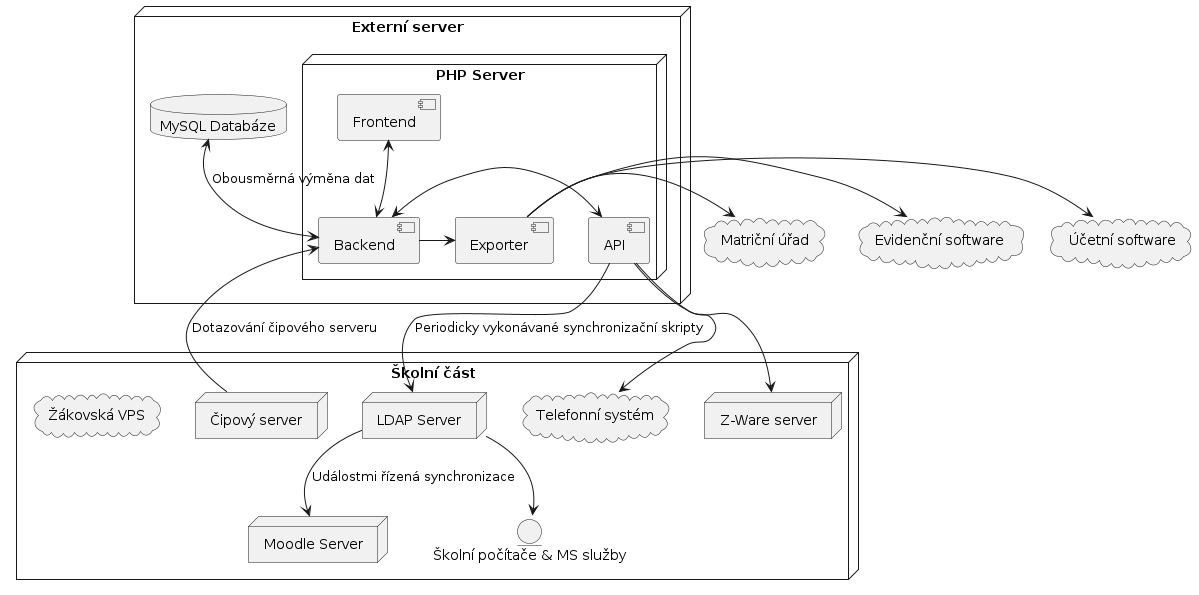
\includegraphics[width=\linewidth]{architektura-puvodni.png}
        \caption{Stávající architektura IS. Zelené komponenty jsou
        spravovány školou, červené externí službou.}
        \label{fig:puvodni-architektura}
    \end{figure}
\end{landscape}

Schéma mapuje klíčové komponenty a jejich vzájemné vztahy. Propojení \ref{section:backend-a-frontend}
\nameref{section:backend-a-frontend}, které představuje interakci mezi serverovou logikou a uživatelským
rozhraním. Těsně spjatý s touto částí je vztah mezi \ref{section:backend-a-exporter} 
\nameref{section:backend-a-exporter}, jenž se zaměřuje na export dat z backendového zpracování. 
Následuje \ref{section:backend-a-cipovy-server} \nameref{section:backend-a-cipovy-server}, což je klíčový 
vztah pro řízení příchodů a odchodů žáků do školy. Další, důležitým vztahem je \ref{section:backend-a-api} 
\nameref{section:backend-a-api}, které umožňuje integraci s dalšími systémy a aplikacemi. 
\ref{section:ldap-server-a-moodle} \nameref{section:ldap-server-a-moodle} přestavují spojení mezi 
autentizačním serverem a e-learningovou platformou, a nakonec \ref{section:ldap-server-a-skolni-pocitace} 
\nameref{section:ldap-server-a-skolni-pocitace}, sloužící pro správu přihlašovacích údajů do školních počítačů.


% Kdo za co odpovídá

% Co musím mít a co by chceme mít
% Sequence diag
% nejvyšší vrstva popisu databáze
% Kdo db dělá? jak by byl proces přidání nové komponenty?

\subsection*{Popis architektury stávajícího systému}

Při pohledu na architekturu tohoto ŠIS, lze vidět kombinaci vnějších a vnitřních služeb,
které spolu komunikují synchronizace dat mezi všemi službami, které IS poskytuje pro studenty,
rodiče, pedagogy i nepedagogické zaměstnance.

V diagramu jsou komponenty, které škola spravuje a může je přizpůsobit svým potřebám,
zvýrazněny zeleně. Naopak, červeně jsou označeny ty komponenty, které disponují vlastním
komunikačním rozhraním a IS musí být upraven tak, aby umožnil jejich automatickou správu.

Začněme tím, jak je konfigurován externí server.
Na externím serveru se nalézá relační databáze \textit{MySQL}, která slouží k uložení všech  
strukturovaných dat. Tato databáze je napojena na \textit{Backend} část, což je místo, kde probíhá
většina zpracování a řízení dat mezi databází a uživatelským rozhraním. Na tomto serveru je také
\textit{Frontend}, který je zodpovědný za vizuální prezentaci dat studentům, rodičům, pedagogickým i
nepedagogickým zaměstnancům prostřednictvím webového prohlížeče. Na posledním bodu, máme zde \textit{API},
které slouží jako hlavní komunikační kanál mezi zmíněným backendem a dalšími službami,
jako je Moodle nebo LDAP.

Uvnitř školního areálu máme několik dalších klíčových služeb. \textit{LDAP Server}, který je
zodpovědný za centralizovanou autentizaci a autorizaci všech našich uživatelů v rámci školní
sítě a všech školních počítačů, na kterých běží operační systém Windows 10. Dále máme \textit{Moodle Server},
naši hlavní e-learningovou platformu, a \textit{Žákovská VPS}, 
virtuální privátní server pro studenty, na kterých se žáci učí operovat s Linuxovým prostředím,
jako jsou třeba webové aplikace (tj. konfigurace webových serverů), nebo další služby.
Linuxové VPS jsme zvolili na základě dat spolupráce s průmyslem. Naši školní partneři se vyjádřili,
že všichni, až na výjimky v počtu několika jedinců, využívají Linuxové servery pro svůj firemní záměr. 

Přehled o jednotlivých částí a jejich propojení jsem již zmínil. Nyní je třeba analýza jednotlivých rizik architektury.

\subsection*{Problematika Single Point of Failure}
\label{section:problematika-single-point-of-failure}

Jedním z největších rizik v aktuální architektuře je \textit{Single Point of Failure (SPoF)} na straně PHP serveru. 
Pokud by tento server selhal, způsobilo by to výpadek většiny služeb, což by mělo vážné důsledky v celé škále případů. 

Dle architektury z diagramu \ref{fig:puvodni-architektura} je viditelné, že v případě kdy by selhala celá externí část,
školní část může zcela bez problému fungovat s omezeními. LDAP server má vlastní databázový model pro ukládání dat, tedy
přihlášení na školních počítačích na síti nebude téměř vůbec ohroženo. Jediný případ, který mně napadá, je kdyby si uživatel
na externí části změnil heslo/některé údaje a LDAP se nestihl synchronizovat před selháním. To samé platí i pro Moodle
server, který si drží vlastní databázi uživatelů a dalších svých entit pro svou práci.
Třetí entitou ve školní části jsou \textit{Žákovská VPS}, avšak ty nejsou nijak propojena s IS.

Dalším dílem popisu jsou směry komunikace. Schéma znázorňuje, že mezi LDAP serverem a API je jednosměrné, tedy IS
LDAP může úpravy pouze přijímat. Důvod je jednoduchý: jakýkoliv zásah uživatele je zásahem do kritické části 
dat systému. K tomuto rozhodnutí - blokace obousměrné komunikace, vede bezpečnostní politika školy. Jakmile,
by si žák, nebo zaměstnanec mohl upravit například své jméno, upravil by tím citlivý záznam, který se následně
může propsat do matričních záznamů.

Z celého odstavce tedy vyplývá, že architektura kvůli své diverzifikaci je částečně ubráněna proti Single Point of Failure
a škola může i bez jedné či druhé části fungovat v omezeném režimu.

\section{Bezpečnost ŠIS}
\label{section:bezpecnost-sis}
Jak vyplývá z předchozí sekce, bezpečnost ŠIS a konzistence jeho je prioritou a tedy je
zaujat "default-deny" přístup, který má výchozí nastavení pro jakýkoliv přístup, operaci
nebo transakci zakázáno a povoluje explicitně ty operace nebo přístupy, které jsou
nezbytně nutné pro funkčnost systému nebo aplikace.

\subsection*{Jednosměrnost API \& matriční záznamy}  
\label{section:jednosmernost-api-a-matricni-zaznamy}
Centrální jednotkou IS je Externí část schématu, její databázový model a Backend komponenta. Změny ze strany 
jiných služeb by byl těžce kontrolovatelný a náročný ochranu. IS na žádost MŠMT generuje archivační snapshot
svých matričních záznamů o žácích. Jakmile, by žák si například změnil své jméno v některém ze svých subsystémů,
mohla by nastat synchronizační chyba na kterou systém není přípraven a generování dat pro MŠMT by nebyl korektní.

\section{Datové toky mezi komponentami}
\label{section:datove-toky-mezi-komponentami}
\subsection*{Databáze a backend komponenty}
Backendem rozumíme množinu PHP skriptů, které obsluhují hlavní komunikaci mezi 
jednotlivými komponentami IS.
Mezi databázovým serverem a backendem webového serveru dochází k obousměrné výměně
dat. Backendová komponenta je jediná, která má přímý přístup do databázového serveru
a tedy kontroluje veškerá data, která IS shromažďuje, ukládá či poskytuje. Tato
vrstva na bezpečnostní funkci, zajišťuje konzistenci dat díky velkému množství
bezpečnostních procedur. Z backendové komponenty vystupují pouze další 3 komunikační
zdroje.

\subsection{Backend a Frontend}
\label{section:backend-a-frontend}
Uživatelské rozhraní (frontend) webové aplikace komunikuje s backendem přímo, aby získalo
potřebné informace nebo poslalo uživatelské vstupy přímo ke zpracování. Frontend je
tedy jediný způsob jediný způsob, jak přistoupit k datům uživatelsky přívětivou 
formou - formou webové stránky. Celá webová stránka je tedy generována metodou 
Server-Side-Rendering (SSR) - celý obsah stránky je seskládán
PHP skriptem do čisté HTML podoby a celý odeslán webovému clientu. Tento přístup zajišťuje
možnost manipulace s daty bez potřeby veřejného API. Pokud tedy pedagog, žák či 
rodič chce přistoupit například ke známkám žáka, musí jedině přes tuto webovou stránku.
Tento frontend slouží k manipulaci jak s jednotlivými entitami IS, tak i s dávkovými soubory,
které je potřeba zpracovávat při hromadných akcích typu přijímací řízení nebo správa 
maturitních zkoušek.

Ředitel školy zastává názor, že veřejné API je velká bezpečnostní hrozba kvůli možném útokům
žáků. Většina žáků školy studuje obor Informační technologie a jsou tedy technologicky zdatní.
Žákovi tedy by stačilo znát veřejné API a příslušné dispozice výpočetního výkonu k DDoS útoku.
Školní systém se po dobu útoku stane nepoužitelným a zaměstnanci školy nemohou plnohodnotně
pracovat.

Zde se dají zúčastněným zobrazit různé druhy informací. Uvádím 10 nejčastějších zobrazovaných
informačních stránek:
\begin{itemize}
    \item novinky školy;
    \item informace o osobě;
    \item známky;
    \item rozvrhy;
    \item seznamy tříd, žáků, pedagogů, nepedagogických pracovníků, kontakty;
    \item čipové záznamy příchodů a odchodů;
    \item maturitní témata a okruhy;
    \item detailní informace o SPU žáků;
    \item tématické plány předmětů;
    \item žákovské dlouhodobé práce.
\end{itemize}
Samozřejmostí je, že každá informace je řízena uživatelskými právy, tedy každý vidí pouze ty
informace, které ze zákona musí vědět.

\subsection{Backend a Exporter}
\label{section:backend-a-exporter}
V rámci ŠIS hraje klíčovou roli komponenta Exporter. Tento Exporter je implementován
jako PHP skript s metodami, které mají za úkol získávat data z backendové části 
systému prostřednictvím volání specifických metod. Tento přístup zajišťuje efektivní,
flexibilní, bezpečné a deterministické zpracování a extrakci dat potřebných pro různé
externí entity a procesy.

Struktura Exporteru je záměrně navržena, aby umožňovala snadné rozšíření. Přidání
nových exportních metod je jednoduché a nevyžaduje rozsáhlé změny v existujícím kódu.
Každá nová metoda může být specificky přizpůsobena pro generování datových sad
dle konkrétních požadavků a formátů požadovaných různými externími systémy nebo
organizacemi.

Tato modulárnost a adaptabilita Exporteru přestavuje značnou výhodu pro ŠIS. Umožňuje
rychle reagovat na nové požadavky a efektivně podporovat širokou škálu operací
a formátů dat. Výsledkem je robustný a efektivně spravovaný systém, schopný vyhovět
různorodým potřebám. Současný exportér disponuje třemi následujícími metodami
pro export:
\begin{enumerate}
    \item \nameref{section:export-pro-msmt},
    \item \nameref{section:export-pro-evidenci-majetku},
    \item \nameref{section:export-pro-evidenci-pam}.
\end{enumerate}

\subsubsection{Export pro MŠMT}\label{section:export-pro-msmt}
Export dat pro MŠMT, které spravuje matriční 
záznamy žáků ohledně jejich studia, jejich speciálních potřeb a jejich následných vazeb.
Jednou z takových vazeb může být platba státního zdravotního a sociálního pojištění.

MŠMT pořádá 2x ročně tzv. sběr\cite{skolni-matrika}, při kterých si vyžádá od školy,
(tedy ŠIS) snapshot ve formátu XML a se specifickým jménem a formátem o celé řadě 
dat o žácích školy. Každá úroveň státního školství má své specifické datum odevzdání.
Tyto informace poskytuje ministerstvo formou tabulky ve článku na svých stránkách
\cite{msmt-terminy-predavani-dat-2023}. Výjimkou je terciální vzdělávání, které probíhá
především na univerzitách. které se řídí dle SIMS - Sdružené informace matrik studentů.

Snapshot je rozdělen do 3 souborů:
\begin{itemize}
    \item soubor dat \textbf{a} se žáky s SPU,
    \item soubor dat \textbf{b} o podpůrných opatřeních poskytovaných školou žákům,
    \item soubor s intaktními žáky.
\end{itemize}

Struktura souborů je dělena do položek, druhu kódování (tvaru zápisu),
druhu číselníku, typu dat, povolené délce řetězce a povinnost záznamu.
Vybírám těchto deset prvků pro rozmanitost datové sady:
\begin{itemize}
    \item datum sběru;
    \item IZO školy;
    \item rodné číslo žáka;
    \item pohlaví žáka;
    \item okres trvalého bydliště žáka;
    \item kvantifikátor státního občanství;
    \item nejvyšší stupeň vzdělání, kterého žák dosáhl před přijetím ke vzdělávání;
    \item ročník, ve kterém se žák vzděláván;
    \item způsob financování vzdělávání;
    \item kód 1. cizího studovaného jazyka.
\end{itemize}

Struktury souborů dat jsou zvláště specifické pro každou úroveň vzdělávacího procesu, 
od mateřských škol, po vyšší odborné. Naší kategorií je formát pro střední školy.
Počet položek v souboru dat o žácích s SPU 54 \cite{msmt-rozhrani-predavani-dat-2023},
v souboru s podpůrnými opatřeními poskytovaných školou žákům je 24 
\cite{msmt-rozhrani-predavani-dat-2023} a v posledním souboru pro žáky intaktní počet položek
je roven 47 \cite{msmt-rozhrani-predavani-dat-2023}.

Všechna tato data prochází anonymizací na straně školy a tedy MŠMT nemá přesné informace o konkrétních 
žácích, přesto MŠMT musí ověřovat správnost vydaných posudků z PPP nebo SPC. Z dat školy spočítá počet 
zadaných žáků s posudky a konkrétní specifikací a jejich platnost. PPP/SPC tato data, také anonymizovaně 
poskytuje MŠMT. MŠMT vykonává tzv. \textbf{kontrolní součty}, tedy porovnává počet žáků s vydanými posudky
od PPP/SPC pro danou školu a počet žáků, které škola poskytuje. Pokud se tyto počty neshodují, MŠMT
vyjednává opravu dat.

\begin{figure}[H]
    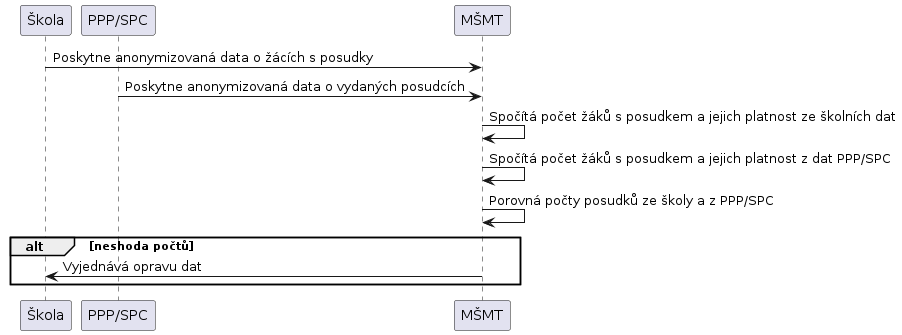
\includegraphics[width=\textwidth-28pt]{seq-kontrolni-soucty.png}
    \caption{Sequence diagram procesu verifikace dat s SPU}
    \label{fig:seq-kontrolni-soucty}
\end{figure}

\begin{figure}[H]
    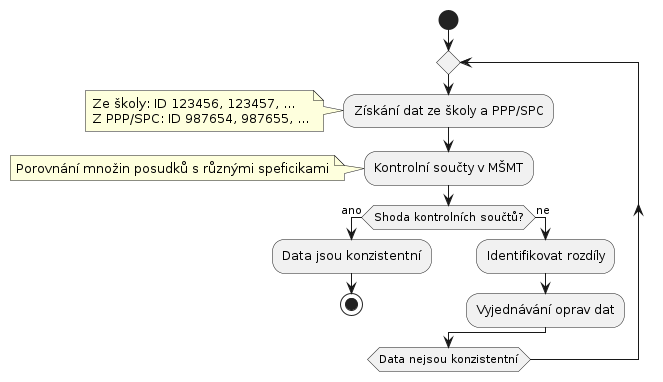
\includegraphics[width=\textwidth-28pt]{act-proces-kontrolnich-souctu.png}
    \caption{Diagram aktivit procesu ověření kontrolních součtů}
    \label{fig:act-proces-kontrolnich-souctu}
\end{figure}

MŠMT dále zpracovává data o všech žácích pro statistické účely a financování. 

Problematikou implementace exporteru se zkomplikovává častou aktualizací datového rozhraní
pro předávání dat. Aktualizaci rozhraní vydává MŠMT přibližně jednou ročně, včetně aktualizace
číselníků \cite{msmt-rozhrani-predavani-dat-2023}. Možnost implementace se ještě zhoršuje kvůli formátu,
ve kterém ministerstvo poskytuje nové aktualizace. Formátem je PDF soubor ve článku na webu, tedy
neexistuje žádný XML soubor, udávající strukturu. Tento způsob tedy potřebuje vždy zásah do implementace
člověkem a je třeba kontaktovat MŠMT, aby konkrétně specifikovalo strukturu.

\subsubsection{Export pro Evidenci majetku} \label{section:export-pro-evidenci-majetku} 
Evidenční software, který je součástí ŠIS, hraje klíčovou roli v řízení a správě fyzického
majetku školy. Exporter zde zastává zásadní úlohu tím, že zajišťuje pravidelnou aktualizaci 
a přenos dat týkajících se školního inventáře, což zahrnuje podrobné informace o zařízeních,
jako jsou počítače, laboratorní vybavení, knihy a další školní zdroje. Tato data jsou 
nezbytná pro efektivní inventarizaci a správu majetku, což umožňuje škole sledovat jeho 
stav, umístění a plánovat případné nákupy nebo údržbu. Evidenční software tak hraje
klíčovou roli v udržení přehledu a efektivního využívání školních zdrojů. 

\subsubsection{Export pro Mzdový a personální software (PaM)} \label{section:export-pro-evidenci-pam}
V oblasti finanční správy je rovněž důležité, aby byla data týkající se zaměstnanců a jejich
úvazků správně zpracována a integrována do Účetního softwaru. Exporter zde poskytuje potřebné
informace pro kalkulaci výplat zaměstnanců. Tato data jsou využívána účetním softwarem pro 
přesné výpočty mzdových nákladů, odvodů a případných příplatků.

Všechna potřebná data pro software k Evidenci majetku a PaM jsou Exporterem vygenerována 
do dávkového souboru a následně nahrána do příslušného softwaru. 

\subsection{Backend a Čipový server}
\label{section:backend-a-cipovy-server}
Propojení Backendu IS s čipovým serverem je důležitý prvek pro sledování přítomnosti
zaměstnanců a studentů ve školním prostředí. Realizováno je to pomocí čipových karet žáků
a 2 záznamových zařízení před vchodem do školy a před východem ze školy. Záznamová zařízení
evidují do databáze čipového serveru čísla přikládaných karet. Přestože čipový 
server je starší technologie, která byla nasazena před více než 25 lety a neobsahuje 
žádné API rozhraní. Aby bylo dosaženo funkčního propojení s novějším Backend systémem,
propojení se realizuje přímým SSH napojením do serveru a poté vybíráním dat ze souborů,
kam systém data ukládá.

IS si eviduje čísla vydaných karet a ta má v databázi přiřazena k jednotlivým osobám,
Díky této vazbě je IS schopen spárovat příchody a odchody s konkrétní osobou. IS si avšak žádná
data nestahuje a vždy se přímo dotazuje. Hlavním přístupovým bodem k datům z příchodů 
a odchodů je webová stránka. Tedy pokud se uživatel dotáže na složitější strukturu dat, typu:
výpis příchodů a odchodů celé třídy, načítání stránky trvá i vyšší jednotky sekund.

\begin{figure}[H]
    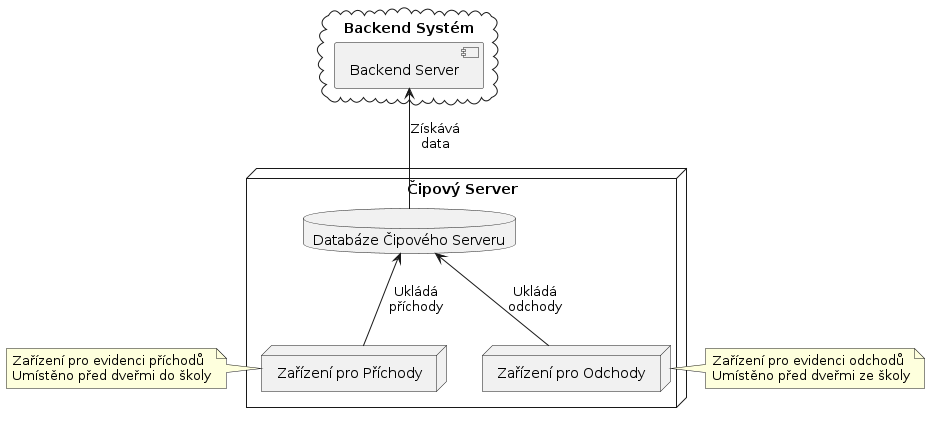
\includegraphics[width=\textwidth-28pt]{backend-cipovy-server.png}
    \caption{Schéma propojení záznamového systému čipových karet}
    \label{fig:backend-cipovy-server}
\end{figure}

\subsection{Backend a API}
\label{section:backend-a-api}
Backend systému je propojen pomocí neveřejného API s dalšími komponentami IS. Skryté API je 
uchováno pod speciální URL adresou se specifickým klíčem. Z tohoto API čerpají interní systémy,
především LDAP server, telefonní systém a Z-Ware.

Telefony (tj. systém telefonů) se dotazuje API pro synchronizaci linek ve škole a zajišťuje 
jejich konfiguraci. LDAP server se synchronizuje s API IS na základě periodicky vykonávaných
skriptů, obvykle 1x denně, případně lze i manuálně při údržbě.

Z-Ware je systém pro školní jídelnu. Ten si synchronizuje data sám, dle svého mechanismu
(garantuje externí firma). Data, která si synchronizuje jsou: čísla karet a čipů a žákovské 
účty, to jsou: username a heslo. Vše ostatní si řídí externí systém Z-Ware sám, včetně volby
obědů, záznamových zařízení, platby za obědy.

\begin{figure}[H]
    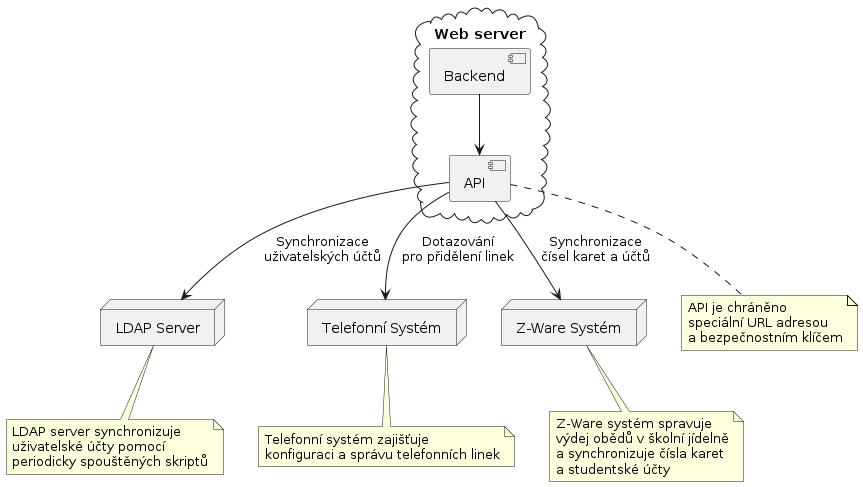
\includegraphics[width=\textwidth-28pt]{backend-api.png}
    \caption{Schéma připojení systémů na API}
    \label{fig:backend-api}
\end{figure}

\subsection{LDAP server a Moodle}
\label{section:ldap-server-a-moodle}
Jednou z dalších částí je komunikace mezi LDAP serverem a Moodle serverem. Moodle je na škole
využíván jako hlavní nástroj pro celý e-learning a tedy je velmi důležitou součástí především
odborných předmětů, kam učitelé umisťují většinu školních úloh nebo domácí úkolů.

Systém Moodle má modul, který umí synchronizovat uživatele a autentifikovat je u LDAP serveru.
To znamená, že pokud se uživatel (žák či zaměstnanec) chce přihlásit do Moodle, ten se 
autentifikuje uživatele LDAP protokolem u LDAP serveru a tím udržuje synchronizované účty právě
při události uživatele.
Vše lze řešit pomocí administrátora Moodle serveru, který může manuálně provést zavedení 
nových účtů a mazání starých či manuální synchronizaci.

Data, která se synchronizují jsou: jména, příjmení, email a třída. Pokud uživatel nemá třídu,
nepřiřazuje se a administrátor musí manuálně identifikovat uživatele. Vše ostatní, jako jsou 
zápisy do kurzů si řeší uživatelé sami. Moodle disponuje i vlastním ověřováním, avšak tento
mechanismus se používá pouze  v ryze výjimečných případech, kdy chceme vytvořit účet i pro 
externí osobu.

\subsection{LDAP server a školní počítače}
\label{section:ldap-server-a-skolni-pocitace}
Veškeré počítače se autentifikují u LDAP serveru na domácí doméně SPSEJECNA.CZ. Jiné účty
na školních počítačích nejsou dovoleny z důvodu bezpečnosti.
Účet na školním Windows počítači se pouze u LDAP serveru autentifikuje. Žákovské, nebo
zaměstnanecké účty se ve škole nijak neliší. Jedinými synchronizovanými daty mezi školními
počítači a serverem jsou uživatelské disky na školních serverech.

% Národní standard spisové e. služby
% cermat není orgán veřejné moci -> nemá povinnost mít spisovku nesplňuji NSESSS
% Pochvala, dutka -> musí mít jednací číslo
% Musí být zadáno do spisové služby

% Katalogový list žáka -> matrika ve škole, neodesílá se
% identifátor subjektu vzdělávání IDSV -> do 2030

\section{Aplikace funkcionalit v informačním systému}
V rámci implementace IS, který je specificky navržen pro potřeby konkrétního školního prostředí,
byla začleněna řada klíčových funkcionalit, které jsou zásadní pro efektivní a plynulý provoz
instituce. Tento systém, jak je znázorněno v diagramu \ref{fig:puvodni-architektura},
zahrnuje různé komponenty, každý se specifickými úkoly a odpovědnostmi. Níže jsou uvedeny
hlavní funkcionality a Ječná IS a jejich implementace v rámci systému.

\subsection*{Správa žákovské agendy}
Správa žákovské agendy v IS zahrnuje shromažďování, spravování a uchovávání žákovských
záznamů, včetně osobních údajů, výsledků studia a docházky. Tato funkcionalita je realizována
prostřednictvím záznamů v databázi, zpracovávání pomocí komponenty Backend a úpravy skrze
Frontendové prostředí. Tyto komponenty jsou vyznačeny v diagramu zeleně, což ukazuje na jejich
spravovatelnost a přizpůsobitelnost dle potřeb školy.

\begin{figure}[H]
    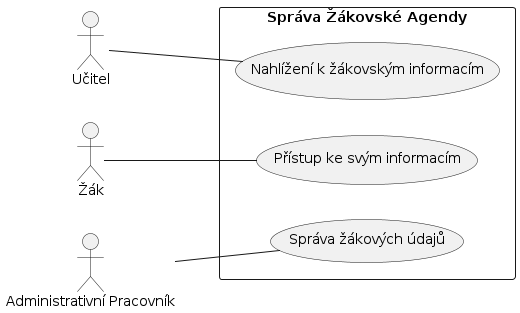
\includegraphics[width=\textwidth-28pt]{uc-sprava-zakovske-agendy.png}
    \caption{Use Case diagram Správy žákovské agendy}
    \label{fig:uc-sprava-zakovske-agendy}
\end{figure}

\subsection*{Integrace přijímacího řízení}
Funkcionalita integrace přijímacího řízení poskytuje nástroje pro správu přijímacích procesů,
včetně přihlášek, evidence uchazečů, evaluace přijatých, přiřazení a vytvoření nových účtů.
V našem IS je tato funkce podporována, což umožňuje škole ušetřit mnoho administrativní zátěže.
Tato funkcionalita je implementována v Frontendu formou formuláře, kde se dále zpracovává v 
Backendu a ukládá v databázi.

\begin{figure}[H]
    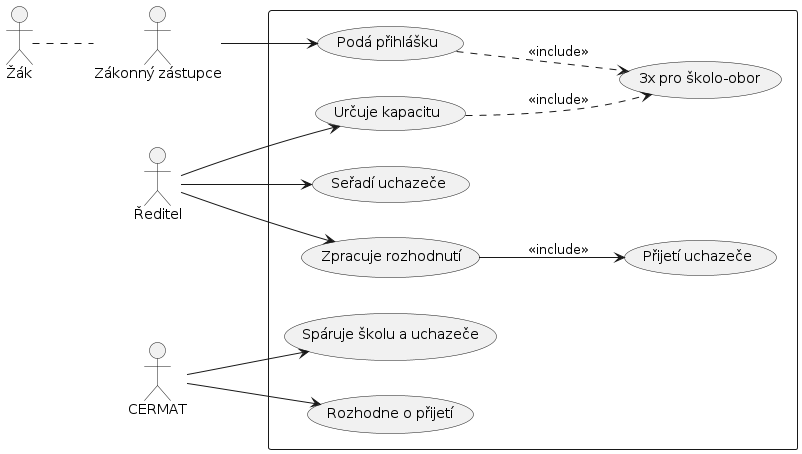
\includegraphics[width=\textwidth-28pt]{uc-integrace-prijimaciho-rizeni.png}
    \caption{Use Case diagram Integrace přijímacího řízení}
    \label{fig:uc-integrace-prijimaciho-rizeni}
\end{figure}

\begin{figure}[H]
    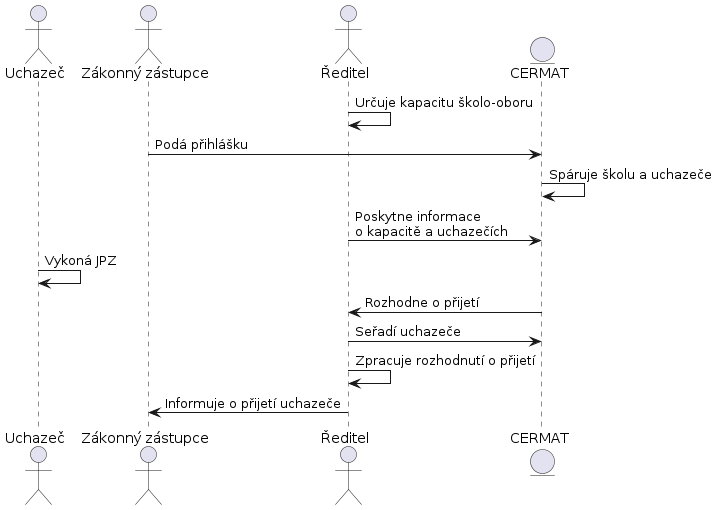
\includegraphics[width=\textwidth-28pt]{seq-integrace-prijimaciho-rizeni.png}
    \caption{Sequence diagram Integrace přijímacího řízení}
    \label{fig:seq-integrace-prijimaciho-rizeni}
\end{figure}

\subsection*{Správa hodnocení}
Správa hodnocení umožňuje učitelům zaznamenávat, sledovat a analyzovat výsledky žáků. Tato
funkcionalita je zásadní pro poskytovaní zpětné vazby žákům a pro monitorování jejich výkonu.
V našem IS je tato funkcionalita implementována jako jedna ze základních položek a je 
implementována formou tabulek a formulářů na straně Frontendu, zpracováván v Backendu a
ukládán v databázi.

\begin{figure}[H]
    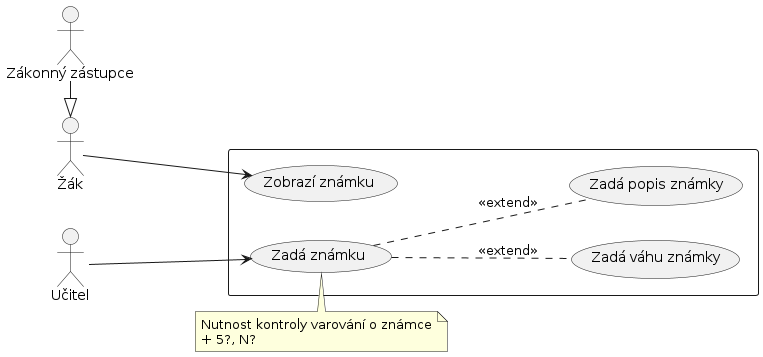
\includegraphics[width=\textwidth-28pt]{uc-sprava-hodnoceni.png}
    \caption{Use Case diagram Správa hodnocení}
    \label{fig:uc-sprava-hodnoceni}
\end{figure}

Škola v informačním systému, zakládá 2 další hodnotící stupně kromě standardních 
v českém školství (hodnotící stupně 1-5). Těmito známkami jsou: \textbf{N?} 
a \textbf{5?}. Tyto známky se udávají do systému jako výchovná opatření,
avšak na vysvědčení psána nikdy není. Známky jsou udávány jako varování za 
zaostávání ve studiu (\textbf{5?}) či varování na neklasifikaci (\textbf{N?}).

\subsection*{Digitální evidence SPU}
Správa specifických poruch učení (SPU) žáků je součástí IS. Tato funkcionalita umožňuje
výchovným poradkyním evidovat zprávy ze zdravotních ústavů: Pedagogicko-psychologické 
poradny (PPP) nebo Speciálního pedagogického centra (SPC). Tyto informace
jsou zpracovány výchovnými poradkyněmi a ve zpracované formě včetně doporučení úpravy
výuky jsou zpřístupněny pedagogům, kteří daného žáka vyučují. Toto je klíčové pro
správné a efektivní fungování inkluzivního a adaptivního vzdělávacího prostředí.
Implementace je pomocí Frontendu, Backendu pro zpracování a databáze pro ukládání.

\begin{figure}[H]
    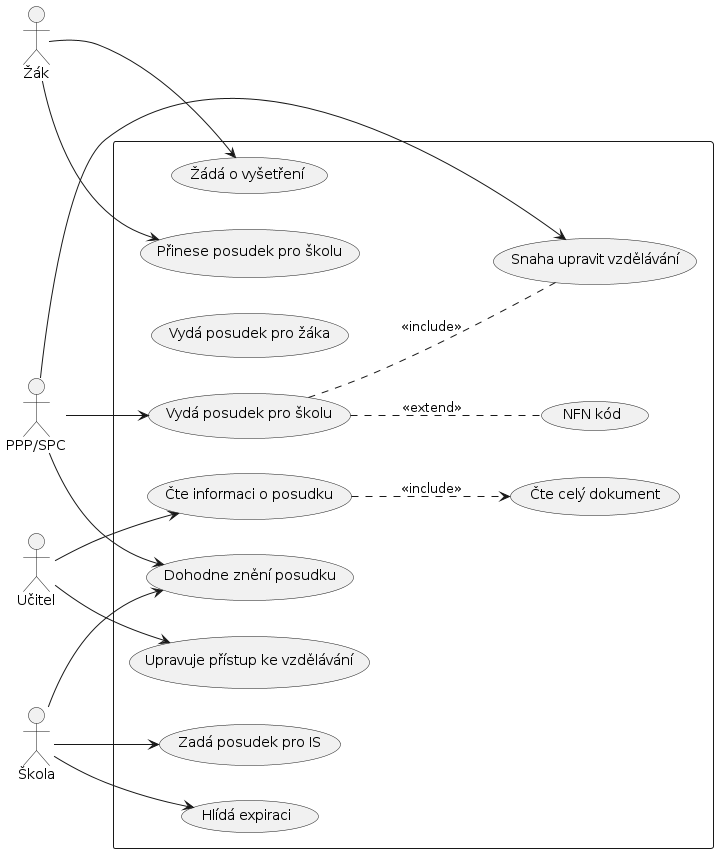
\includegraphics[width=\textwidth-28pt]{uc-digitalni-evidence-spu.png}
    \caption{Use Case diagram Digitální evidence SPU}
    \label{fig:uc-digitalni-evidence-spu}
\end{figure}

Právem každé školy je kontrola znění posudku. Škola kontrolu vyžaduje, aby se předešlo
nedorozuměním ve špatném výkladu a spravedlivému, praktickému přizpůsobení výuky
v konzultaci pracovníka vydavatele posudku s odborníky v oboru.

\begin{figure}[H]
    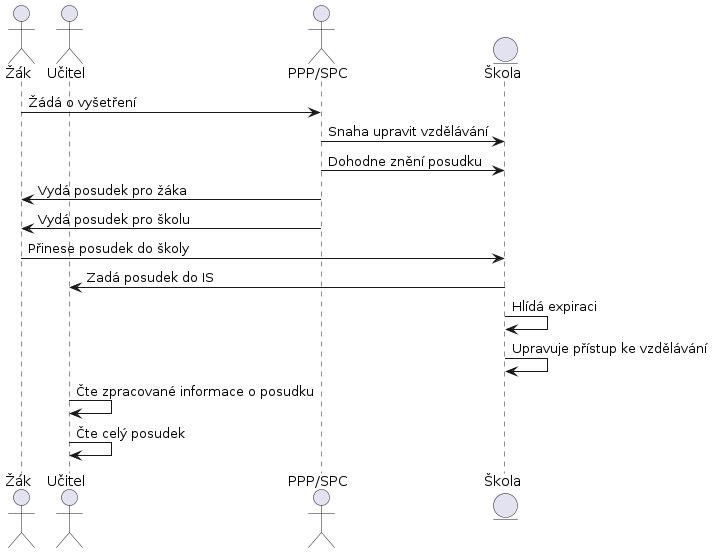
\includegraphics[width=\textwidth-28pt]{seq-digitalni-evidence-spu.png}
    \caption{Sequence diagram Digitální evidence SPU}
    \label{fig:seq-digitalni-evidence-spu}
\end{figure}

\subsection*{Centrální hlášení závad}
Ječná IS zahrnuje funkcionalitu pro centrální evidenci závad ve škole, který umožňuje
žákům a zaměstnancům hlásit a spravovat technické problémy nebo závady ve škole.
Implementován je pomocí služeb Microsoftu, tedy veřejný email, který ukládá informace
a distribuuje mezi správce školní sítě a vedení školy.

\begin{figure}[H]
    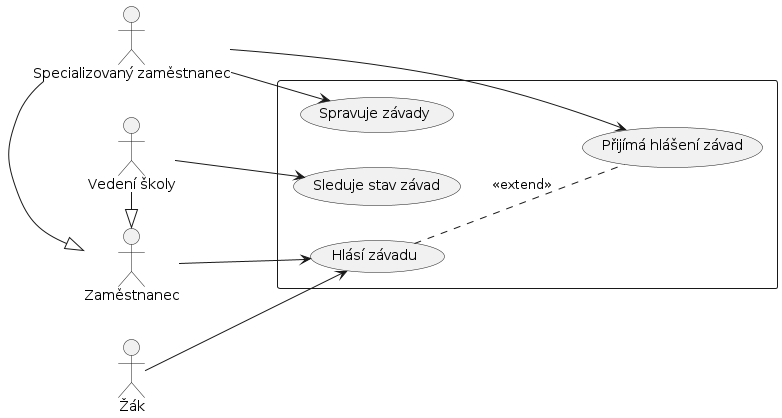
\includegraphics[width=\textwidth-28pt]{uc-centralni-hlaseni-zavad.png}
    \caption{Use Case diagram Centrální hlášení závad}
    \label{fig:uc-centralni-hlaseni-zavad}
\end{figure}

\subsection*{Správa absencí}
Funkcionalita správy absencí zajišťuje přehled o docházce studentů a umožňuje identifikaci
a řešení problémů s absencemi. Tato funkcionalita je v IS plně podporována je jedna ze 
základních položek. Implementována je pomocí tabulek a formulářů na Frontendu, spravována 
Backendem a ukládána do databáze.

\begin{figure}[H]
    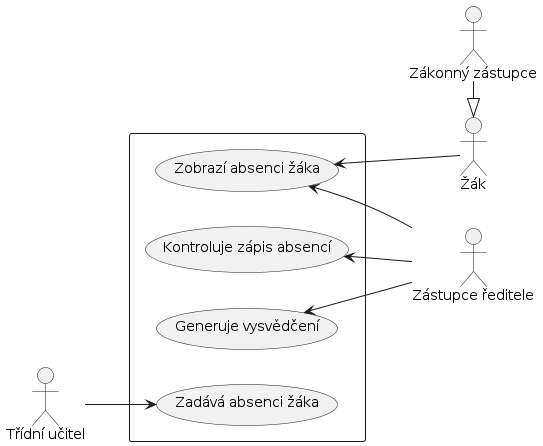
\includegraphics[width=\textwidth-28pt]{uc-sprava-absenci.png}
    \caption{Use Case diagram Správa absencí}
    \label{fig:uc-sprava-absenci}
\end{figure}

V diagramu je znázorněno, že absenci žáka zadává třídní učitel a žák s zákonným zástupcem
si absenci mohou zobrazit. V IS není nijak implementováno, že by zákonný zástupce mohl
absenci omluvit. Toto je řešeno papírovým omluvným listem z důvodu bezpečnosti. Dle zkušeností
je velmi snadné pro žáky přistoupit k účtu zákonného zástupce a omluvit se sám, což není žádané.

\subsection*{Dokumentový management}
Dokumentový management v našem systému plní funkci úložiště veřejných dokumentů
a dokumentů pro školu. Dělí se na následující sekce:
\begin{itemize}
    \item pro veřejnost;
    \item pro žáky a rodiče;
    \item pro vedení;
    \item pro zaměstnance;
    \item fotografie z akcí.
\end{itemize}
Do jednotlivých sekcí mohou ukládat soubory pouze zaměstnanci, kteří mají k
přesně tomuto účelu speciální právo v systému pravomocí k IS. Zobrazení dané 
sekce je omezeno též speciálními právy. Dvěmi sekcemi, které jsou k dispozici
široké veřejnosti jsou: Fotografie z akcí a Pro veřejnost. V první sekci se
nalézají veškeré reprezentativní fotografie z akcí a též systém novinek na 
úvodní stránce z této složky čerpá. Druhá sekce disponuje prezentačními materiály
školy, školními dokumenty, které musí škola vydávat veřejně.
Implementován je pomocí Backendu, který uděluje práva uživatelům IS a manipuluje 
s daty. Vše je zobrazováno ve Frontendu pomocí seznamu souborů file-systému, kde
se stahují všechny dokumenty HTTP protokolem na přímou žádost o stažení dokumentu.

\subsection*{Certifikace}
Funkcionalita certifikace v Ječná IS umožňuje sledování a správu 
certifikací a kvalifikací získaných žáky nebo personálem. Tato funkce je důležitá
pro dokumentaci a uznání úspěchů, kterými jsou odborné certifikáty. Díky této 
správě lze jednoduše zjistit, jací žáci mají složenou odbornou zkoušku, 
která by žákům mohla zajistit odpuštění praktické části zkoušky maturitní.
Funkcionalita je implementována pomocí tabulek na Frontendu, zpracováním na Backendu
a ukládáním v databázi.

\begin{figure}[H]
    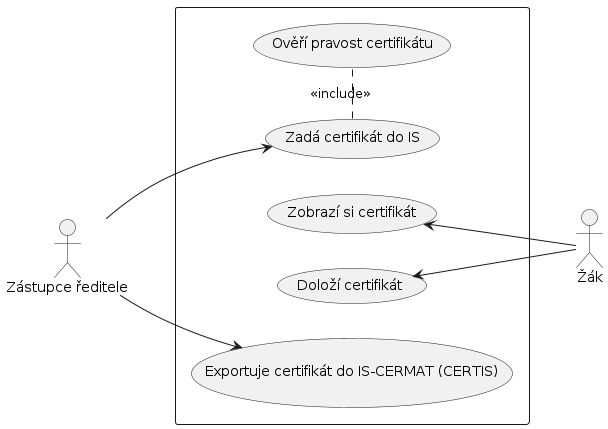
\includegraphics[width=\textwidth-28pt]{uc-certifikace-zaku.png}
    \caption{Use Case diagram Certifikace žáků}
    \label{fig:uc-certifikace-zaku}
\end{figure}

\begin{figure}[H]
    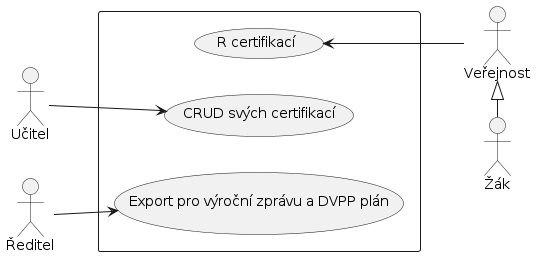
\includegraphics[width=\textwidth-28pt]{uc-certifikace-zamestnancu.png}
    \caption{Use Case diagram Certifikace zaměstnanců. CRUD = Create, Read, 
             Update, Delete}
    \label{fig:uc-certifikace-zamestnancu}
\end{figure}

\subsection*{Správa vzdělávacích plánů}
Správa tématických plánů  je zásadní pro organizaci a plánování vzdělávacího obsahu.
Tato funkcionalita umožňuje učitelům vytvářet, upravovat a spravovat tématické plány
pro různé předměty. Efektivní správa těchto plánů podporuje jasnou evidenci vyučovaných
témat týden po týdnu pro celý školní rok. Implementace je realizována pomocí tabulek
na Frontendu, zpracování na Backendu a ukládáním v databázi.

\begin{figure}[H]
    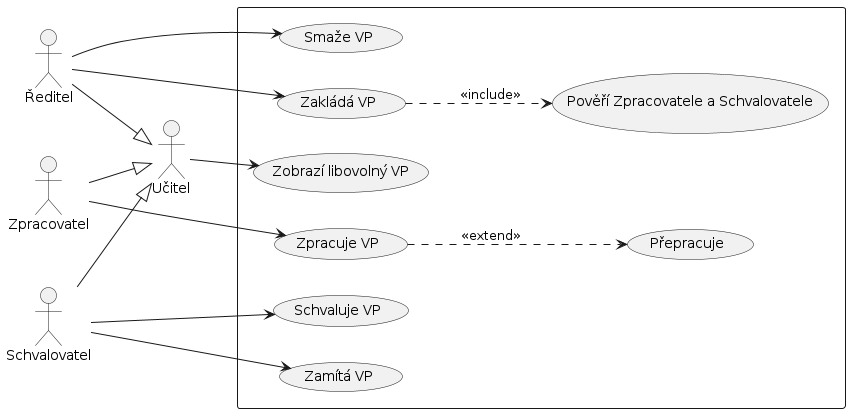
\includegraphics[width=\textwidth-28pt]{uc-sprava-vzdelavacich-planu.png}
    \caption{Use Case diagram Správy vzdělávacích plánů. VP = Vzdělávací plán}
    \label{fig:uc-sprava-vzdelavacich-planu}
\end{figure}

\begin{figure}[H]
    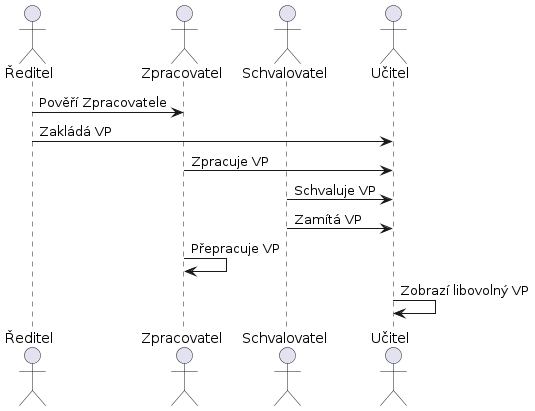
\includegraphics[width=\textwidth-28pt]{seq-sprava-vzdelavacich-planu.png}
    \caption{Sequence diagram Správy vzdělávacích plánů. VP = Vzdělávací plán}
    \label{fig:seq-sprava-vzdelavacich-planu}
\end{figure} 

\subsection*{Matriční záznamy}
Důležitost evidence a exportu matričních záznamů je již vysvětlena v sekci 
\ref{section:backend-a-exporter}. Systém je implementován pomocí Exporteru, 
který generuje dávkové soubory, Backendu, který zpracovává komunikaci a databází
pro získávání dat.


\section{Databázový server a databázový model}
Současná databáze IS využívá MySQL verze 8.0.32 a její model celkem disponuje 76 entitami,
každá přidružená k některé z kategorií funkcionalit, které IS disponuje. Jediným správcem 
databáze v současné době je současný správce IS, ředitel školy. 
Veškerá dokumentace je již vytvořena a udržována ve formě papírového spisu a elektronických
dat v budově školy.

%\begin{table}[H]
%\begin{tabular}{lcl}
%\hline
%\multicolumn{1}{|l|}{\textbf{Druh}}                  & \multicolumn{1}{c|}{\textbf{Počet}} & \multicolumn{1}{l|}{\textbf{Užití}}                                                                                                                                       \\ \hline
%\multicolumn{1}{|l|}{Žákovská správa}                & \multicolumn{1}{c|}{16}             & \multicolumn{1}{l|}{\begin{tabular}[c]{@{}l@{}}Identifikační údaje, rodiče, absence,\\ třídy, skupiny, certifikace, zdravotní\\ záznamy, specifické potřeby\end{tabular}} \\ \hline
%\multicolumn{1}{|l|}{Zaměstnanecká správa}           & \multicolumn{1}{c|}{5}              & \multicolumn{1}{l|}{\begin{tabular}[c]{@{}l@{}}Identifikační údaje, typ úvazku,\\ třídnictví, kabinet\end{tabular}}                                                       \\ \hline
%\multicolumn{1}{|l|}{Správa rozvrhů}                 & \multicolumn{1}{c|}{3}              & \multicolumn{1}{l|}{\begin{tabular}[c]{@{}l@{}}Úvazky zaměstnanců, rozvrhy \\ učeben, rozvrhy tříd\end{tabular}}                                                          \\ \hline
%\multicolumn{1}{|l|}{Správa budovy}                  & \multicolumn{1}{c|}{2}              & \multicolumn{1}{l|}{\begin{tabular}[c]{@{}l@{}}Kabinety, učebny, technické místnosti,\\ kanceláře, správa kanceláří\end{tabular}}                                         \\ \hline
%\multicolumn{1}{|l|}{Správa předmětů}                & \multicolumn{1}{c|}{5}              & \multicolumn{1}{l|}{Předměty, akreditace, tématické plány}                                                                                                                \\ \hline
%\multicolumn{1}{|l|}{Správa souborového systému}     & \multicolumn{1}{c|}{3}              & \multicolumn{1}{l|}{\begin{tabular}[c]{@{}l@{}}Soubory k novinkám, certifikáty,\\ administrativní dokumenty\end{tabular}}                                                  \\ \hline
%\multicolumn{1}{|l|}{Správa informací pro veřejnost} & \multicolumn{1}{c|}{3}              & \multicolumn{1}{l|}{\begin{tabular}[c]{@{}l@{}}Novinky, informace k přijímacímu \\ řízení, školní akce\end{tabular}}                                                      \\ \hline
%\multicolumn{1}{|l|}{Správa školních akcí}           & \multicolumn{1}{c|}{4}              & \multicolumn{1}{l|}{\begin{tabular}[c]{@{}l@{}}Elektronické přihlašování na akce \\ pořádané školou\end{tabular}}                                                         \\ \hline
%\multicolumn{1}{|l|}{Správa maturitních zkoušek}     & \multicolumn{1}{c|}{8}              & \multicolumn{1}{l|}{\begin{tabular}[c]{@{}l@{}}Data, účasti, místnosti, přepis \\ místností, maturitní projekty\end{tabular}}                                             \\ \hline
%\multicolumn{1}{|l|}{Správa přijímacího řízení}      & \multicolumn{1}{c|}{2}              & \multicolumn{1}{l|}{\begin{tabular}[c]{@{}l@{}}Identifikační údaje, kola, ukončené\\ vzdělání, studijní výsledky\end{tabular}}                                            \\ \hline
%\multicolumn{1}{|l|}{Spolupráce s průmyslem}         & \multicolumn{1}{c|}{2}              & \multicolumn{1}{l|}{\begin{tabular}[c]{@{}l@{}}Nabídky prací pro žáky, \\ spolupráce s průmyslem\end{tabular}}                                                            \\ \hline
%\multicolumn{1}{|l|}{Číselníky MŠMT a NUTS}          & \multicolumn{1}{c|}{15}             & \multicolumn{1}{l|}{\begin{tabular}[c]{@{}l@{}}Číselníky pro předávání \\ individuálních údajů ze školních\\ matrik státní správě, nomenklatura \\územních statistických jednotek\end{tabular}}                           \\ \hline
%\multicolumn{1}{|l|}{Ostatní}                        & \multicolumn{1}{c|}{6}              & \multicolumn{1}{l|}{\begin{tabular}[c]{@{}l@{}}Číselné kódy zemí, anonymizační\\ číselníky, variabilní symboly bank \\bezpečnostní evidence\end{tabular}}                                         \\ \hline
%\multicolumn{1}{r}{\textbf{SUMA}}                    & 74                                  &                                                                                                                                                                          
%\end{tabular}
%\caption{Evidence druhů entit v relačním modelu databáze}
%label{analysis:db-model}
%\end{table}

%top\newpage

\chapter{Diskuse}
\section{Porovnání výsledků s původními hypotézami a otázkami práce}
Analýza současného stavu ŠIS ukázala, že in-house vývoj poskytuje vysokou míru 
komplexnosti a integrace kritických funkcí. Tyto funkce, které jsou zásadní pro 
efektivní správu školy, nejsou vždy plně pokryty dostupnými komerčními systémy.
Ekonomická kalkulace přechodu na jiný systém by proto měla zahrnovat nejenom náklady 
na pořízení nového systému, ale také potenciální ztrátu specifických funkcionalit,
které současný IS poskytuje.

Přechod na komerční ŠIS by mohl přinést významné náklady spojené s migrací dat,
školením personálu a adaptací na nový systém. Navíc ztráta klíčových funkcí
by mohla mít negativní dopad na provoz školy, jako například ztížení administrativních
procesů, nebo snížení efektivity komunikace mezi zaměstnanci a studenty.

\section{Ekonomická kalkulace a diskuze}
\subsection{Přechod na systém Bakaláři}
Za předpokladu přechodu na systém Bakaláři je třeba započítat náklady na migraci dat,
školení personálu, upravení subsystémů, které by byly jednorázové. Dále je třeba 
započítat náklady na licenci, která se platí ročně.

\begin{table}[H]
    \centering
    \begin{tabular}{lccc}
    \multicolumn{1}{c}{\textbf{Druh nákladu}}                                                           & \begin{tabular}[c]{@{}c@{}}Délka výkonu \\ {[}den{]}\end{tabular} & Man-day              & \begin{tabular}[c]{@{}c@{}}Skutečná \\ cena\end{tabular} \\ \hline
    \textbf{Migrace dat}                                                                                & 5                                                                 & 12000                & 60000                                                    \\
    \textbf{Rekonfigurace školních subsystémů}                                                          & 5                                                                 & 2500                 & 12500                                                    \\
    \textbf{Lektor pro školení pedagogů}                                                                & 1                                                                 & 2500                 & 2500                                                     \\
    \textbf{\begin{tabular}[c]{@{}l@{}}Lektor pro školení \\ specializovaných zaměstnanců\end{tabular}} & 1                                                                 & 2500                 & 2500                                                     \\
    \textbf{Lektor pro školení vedení školy}                                                            & 1                                                                 & 2500                 & 2500                                                     \\ \hline
    \textbf{SOUČET}                                                                                     & 13                                                                & \multicolumn{1}{l}{} & 80000                                                   
    \end{tabular}

    \caption{Tabulka ekonomické kalkulace přechodu na systém Bakaláři. 
    Délky úkonů a ceny práce (Man-day) jsou odhadnuty.}
    \label{analysis:ekonomicka-kalkulace-prechod-bakalari}
\end{table}

Z tabulky \ref{analysis:ekonomicka-kalkulace-prechod-bakalari} práce je možné vyčíst,
že celková cena přechodu na IS bakaláři by byla 80 000 Kč. Do této částky nespadá 
přeprogramování subsystémů, které na současném IS běží, pouze rekonfiguraci.

% https://www.platy.cz/platy/informacni-technologie/databazovy-administrator
% (44294+98135)/2 = 71214.5
% 160hod/mo -> 71214.5/160 = 445.09
% https://www.mesec.cz/clanky/platy-ucitelu-narust/
% 46843/160 = 292.76
% V této kalkulaci předpokládáme, že migrace dat proběhne v rámci 40 hodin 3 zaměstnanců,
% kterým bude vyplácen průměrná mzda v oboru IT, který se pohybuje od 45 360 Kč do
% 114 784 Kč \cite{platy-it}. Pro výpočet průměrné hodinové mzdy použijeme průměr těchto
% hodnot a pro přepočet na hodinovou mzdu vydělíme průměrnou měsíční mzdu počtem hodin,
% tj. 160.
% 
% \begin{samepage}
% Pro výpočet je použit vzorec
% $$\frac{MIN\ CENA + MAX\ CENA}{2*POCET\ HODIN} = CENA\ PRACE$$
% 
% Což při aplikaci je:
% $$\frac{45\ 360 + 114\ 784}{2*160} = 500,45$$
% \end{samepage}
% 
% Cena průměrné hodinové mzdy učitele je vypočtena z průměrné mzdy učitele, tedy 46 843 Kč
% \cite{platy-skolstvi}, která je přepočtena na hodinovou mzdu vydělenou počtem pracovních
% hodin v měsíci.
% 
% \begin{samepage}
%     Pro výpočet je použit vzorec
%     $$\frac{MESICNI\ MZDA}{POCET\ HODIN} = CENA\ PRACE$$
%     
%     Což při aplikaci je:
%     $$\frac{46\ 843}{160} = 292,76$$
% \end{samepage}
% 
% Počet osob na migraci dat je odhadnut na 3. K rekonfiguraci jsou započteni koordinátoři 
% ICT, správce sítě a jeden člen vedení školy s technickou způsobilostí a přehledem o IS.
% Počet pedagogů je zadán na základě výroční zprávy školy ze školního roku 2022/2023 
% \cite{spsejecna-vyrocni-zprava-2022-2023}, tedy 72. Specializovaní zaměstnanci se 
% aktuálně skládají z 22 třídních učitelů, metodikovi prevence, 2 výchovných poradců, 
% 2 koordinátorů ICT, koordinátorovi ŠVP, správci sítě o celkovém počtu 29.
% Počet členů vedení školy je 6: ředitel školy, 3 zástupci ředitele a 2 výchovné poradkyně.
% 
% V celé kalkulaci předpokládáme, že migrace dat bude prováděna externě, mimo pracovníky
% školy. Toto je z důvodu, že škola nemá dostatek kapacit pro provádění této činnosti.
% Rekonfigurace školních systémů je v rámci správce ICT či správce sítě a tedy 
% předpokládáme průměrnou mzdu pedagogického pracovníka pro jednoduchost výpočtu.
% To samé platí pro specializovaných zaměstnanců a vedení školy.

% V tabulce \ref{analysis:ekonomicka-kalkulace-prechod-bakalari} jsou uvedeny výsledky 
% ekonomické kalkulace přechodu na systém Bakaláři. Celkové jednorázové náklady činí 
% 362 918,96 Kč.

\subsection{Zachování současného IS}
V rámci uvažování o budoucím směřování Ječná IS stojí za zvážení varianta udržení stávajícího 
systému s cíleným doplněním nových funkcionalit. Tento přístup vyžaduje evaluaci a porovnání 
stávajícího systému s referenčními systémy, zejména s IS Bakaláři, a stanovení priorit 
v kontextu aktuálních a budoucích požadavků školního prostředí.

V následující tabulce jsou prezentovány prioritní oblasti pro doplnění nebo vylepšení
ve stávajícím IS, s ohledem na jejich kritický význam pro efektivní fungování školy.

\begin{table}[H]
    \centering
    \begin{tabular}{|l|c|}
    \hline
    \textbf{FUNKCIONALITA/IS}  & \textbf{Ječná IS} \\ \hline
    Integrace spisových služeb & \ccrossmark        \\ \hline
    Suplování                  & \textbf{3}        \\ \hline
    Zamlouvání učeben          & \ccrossmark        \\ \hline
    Správa žákovských skupin   & \textbf{4}        \\ \hline
    Elektronická třídnice      & \textbf{2}        \\ \hline
    Offline režim              & \ccrossmark        \\ \hline
    Responzivní design         & \textbf{1}        \\ \hline
    Mobilní aplikace           & \ccrossmark        \\ \hline
    \end{tabular}
    \caption{Neimplementované požadavky v Ječná IS proti IS Bakaláři. 
    Čísla označují prioritu, kde 1 je nejvyšší.}
    \label{analysis:priorities}
\end{table}

Po důkladné analýze a porovnání stávajícího informačního systému Ječná IS 
s referenčním systémem Bakaláři, byly identifikovány klíčové funkcionality,
které absentují v současném systému Ječná IS nebo nedostatečně rozvinuté.
Tabulka \ref{analysis:priorities} poskytuje přehled těchto funkcionalit 
a jejich stanovených priorit, což je zásadní pro určení směru budoucího
rozvoje IS. Prioritizace těchto funkcí reflektuje nejen aktuální požadavky
a potřeby školního prostředí, ale také zohledňuje potenciál pro zvýšení 
efektivity a celkové funkčnosti systému.

V následujícím dependency diagramu je podrobně ilustrována síť závislostí
a vzájemných vztahů mezi funkcionalitami, které jsou nezbytné pro úspěšnou
implementaci elektronické třídnice v IS Ječná. Diagram nejenže zobrazuje 
logické propojení mezi jednotlivými funkcemi, ale také slouží jako vizuální 
reprezentace důvodů stanovení jejich priorit. Elektronická třídnice zde 
figuruje jako základní prvek, jehož efektivní fungování je závislé na 
úspěšné integraci dalších funkcí, jako jsou suplování a správa žákovských skupin. 
Diagram poskytuje hlubší porozumění proč konkrétní funkce byly prioritizovány.

\begin{figure}[H]
    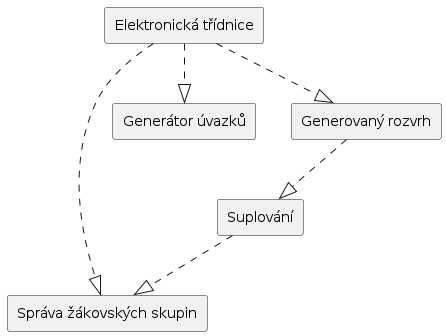
\includegraphics[width=\textwidth-28pt]{dep-eltridnice.png}
    \caption{Dependency diagram funkcionalit}
    \label{fig:dep-eltridnice}
\end{figure}

Následuje rozbor jednotlivých funkcionalit, které jsou byly vyhodnoceny jako prioritní:
\begin{itemize}
    \item \textbf{Responzivní design:} Vzhledem k rostoucí diverzifikaci zařízení používaných
    jak studenty, tak učiteli, se responzivní design jeví jako zásadní pro zajištění univerzální
    přístupnosti IS. Tento prvek je klíčový pro implementaci dalších potřebných funkcionalit z
    hlediska efektivity. Nové prvky v IS již budou v novém vzhledu a nebude poté potřeba 
    redesignovat nedávno implementované.

    \item \textbf{Elektronická třídnice:} Digitalizace třídních záznamů a administrativních 
    procesů je nezbytná pro zefektivnění vzdělávacího procesu a pro poskytují aktuálních informací
    přímo na webu, nikoliv v papírových sešitech.

    \item \textbf{Suplování:} Efektivní řešení pro suplování je klíčové pro implementaci 
    elektronické třídnice. Nelze evidovat odučené učivo v nekonzistentních a nesprávných datech.

    \item \textbf{Správa žákovských skupin:} Žákovské skupiny jsou podmnožinou tříd. Jejich 
    správa žákovských skupin je opět nutná pro elektronickou třídnici pro zajištění správnosti
    a konzistence záznamů. Také podporuje individualizovaný přístup k výuce a umožňuje 
    efektivnější alokaci vzdělávacích zdrojů.
\end{itemize}

Další dvě funkcionality nebyly nativně vyhodnoceny jako priority, protože jsou součástí 
funkcionality: Elektronická třídnice.
\begin{itemize}
    \item \textbf{Generátor úvazků:} V současné době je třeba od všech pedagogů získat data
    o zájmu velikosti úvazku (počet odučených hodin za týden) a žádostí o úpravu rozvrhu na 
    další školní rok. Tato data jsou ručně kontrolována a evidována. Následně se přiřazují 
    předměty, třídy a hodiny jednotlivým učitelům na získaných dat o úvazku základě kompetencí
    pedagoga. Toto by bylo avšak možné automatizovat a úvazky na základě získaných generovat.

    \item \textbf{Generovaný rozvrh:} Nyní se rozvrh ručně vytvoří v dedikovaném programu a 
    následně se nahraje do IS. Pro elektronickou třídnici bude třeba vytvořit rozvrh na každý 
    den unikátní, který bude odpovídat týdennímu, navrženému rozvrhu a změnám v suplování.
\end{itemize}

Též několik funkcionalit nebylo vyhodnoceno jako prioritní.
\begin{itemize}
    \item \textbf{Integrace spisových služeb:} Tato funkcionalita slouží k odbourání
    administrativy spojené s vydáváním oficiálních dokumentů, kde musí specializovaný zaměstnanec
    na žádost jiného zaměstnance ručně žádat spisovou službu o vydání evidenčního čísla. Tuto
    funkcionalitu je v plánu implementovat po aktuálních prioritách. 
    \item \textbf{Offline režim:} Tato funkcionalita v současné době nemá žádný racionální 
    smysl. Současná legislativa ukládá řediteli povinnost evakuovat školu již při výpadku
    elektrické energie, protože není možné udržet ani minimální hygienické požadavky jako je 
    tekoucí voda na toaletách. Obdobný problém je i při výpadku Internetu. V současné době může
    výuka fungovat bez Internetu velice omezeně, na určité odborné předměty téměř vůbec. Z těchto
    důvodů nemá smysl implementovat Offline režim, když výuka je též velice omezena. 
    \item \textbf{Mobilní aplikace:} Náklady na vývoj a údržbu současné webové aplikace jsou vysoké
    a tato funkcionalita by byla dalším velkým zdražením provozu. Řešením je Responzivní design,
    který bude dostatečný pro ovládání systému z telefonu při minimálním navýšení prvotních i 
    dalších nákladů na výrobu a údržbu.
\end{itemize}

\chapter{Závěr}
\section{Shrnutí klíčových zjištění}
Tato práce představuje komplexní analýzu ŠIS Ječná a jeho potenciální modernizace. Z analýzy
vyplývá, že zachování a rozšíření stávajícího systému Ječná IS je nejvýhodnější variantou. 
Klíčová zjištění jsou následující:

\begin{itemize}
    \item unikátní vlastnosti Ječná IS: systém nabízí řadu specifických funkcí, 
    které jsou na míru vytvořené školním potřebám, a které nejsou v plné míře obsaženy 
    v konkurenčních systémech;
    \item nutnost modernizace: přestože systém vykazuje unikátní charakteristiky, 
    je zřejmé, že vyžaduje modernizaci, zejména ve smyslu rozvoje responzivního designu,
    a integrace nových klíčových funkcí, jako je suplování a správa žákovských skupin či
    elektronická třídnice;
    \item ekonomická efektivita: analýza ukázala, že i přes počáteční investici do 
    modernizace, je zachování a rozšíření stávajícího Ječná IS ekonomicky efektivnější 
    oproti úplnému přechodu na nový systém, vzhledem k zachování unikátních funkcí a 
    minimalizaci potřeby školení personálu.
\end{itemize}

\section{Závěrečné úvahy a doporučení pro budoucí praxi a práce}
Na základě zjištění vyplývající z analýzy je možné pokračovat v návrhu rozvoje a 
modernizace stávajícího systému Ječná IS. Tento proces by měl zahrnovat:

\begin{itemize}
    \item doplnění chybějících funkcí: zaměřit se na rozvoj a implementaci prioritních funkcí,
    které zvyšují efektivitu a uživatelský komfort, a které jsou klíčové pro moderní 
    školní prostředí;
    \item zaměření na mobilní technologie: rozvíjet responzivní design, aby systém lépe 
    vyhovoval současným trendům a potřebám uživatelů;
    \item budoucí výzkum a vývoj: v dalších pracích se zaměřit na návrh a implementaci 
    nových inovativních řešení, které budou reagovat na neustále se měnící technologické 
    a vzdělávací trendy.
\end{itemize}

Tato práce poskytla základ pro další diskuzi a rozvoj v oblasti školních informačních systémů 
a ukázala, že cesta modernizace stávajícího systému je životaschopnou a efektivní strategií 
pro budoucí rozvoj.

\chapter{Reference}
\printbibliography[heading=none]

\chapter{Přílohy}


\end{document}
